\documentclass[twoside]{book}

% Packages required by doxygen
\usepackage{fixltx2e}
\usepackage{calc}
\usepackage{doxygen}
\usepackage[export]{adjustbox} % also loads graphicx
\usepackage{graphicx}
\usepackage[utf8]{inputenc}
\usepackage{makeidx}
\usepackage{multicol}
\usepackage{multirow}
\PassOptionsToPackage{warn}{textcomp}
\usepackage{textcomp}
\usepackage[nointegrals]{wasysym}
\usepackage[table]{xcolor}

% Font selection
\usepackage[T1]{fontenc}
\usepackage[scaled=.90]{helvet}
\usepackage{courier}
\usepackage{amssymb}
\usepackage{sectsty}
\renewcommand{\familydefault}{\sfdefault}
\allsectionsfont{%
  \fontseries{bc}\selectfont%
  \color{darkgray}%
}
\renewcommand{\DoxyLabelFont}{%
  \fontseries{bc}\selectfont%
  \color{darkgray}%
}
\newcommand{\+}{\discretionary{\mbox{\scriptsize$\hookleftarrow$}}{}{}}

% Page & text layout
\usepackage{geometry}
\geometry{%
  a4paper,%
  top=2.5cm,%
  bottom=2.5cm,%
  left=2.5cm,%
  right=2.5cm%
}
\tolerance=750
\hfuzz=15pt
\hbadness=750
\setlength{\emergencystretch}{15pt}
\setlength{\parindent}{0cm}
\setlength{\parskip}{3ex plus 2ex minus 2ex}
\makeatletter
\renewcommand{\paragraph}{%
  \@startsection{paragraph}{4}{0ex}{-1.0ex}{1.0ex}{%
    \normalfont\normalsize\bfseries\SS@parafont%
  }%
}
\renewcommand{\subparagraph}{%
  \@startsection{subparagraph}{5}{0ex}{-1.0ex}{1.0ex}{%
    \normalfont\normalsize\bfseries\SS@subparafont%
  }%
}
\makeatother

% Headers & footers
\usepackage{fancyhdr}
\pagestyle{fancyplain}
\fancyhead[LE]{\fancyplain{}{\bfseries\thepage}}
\fancyhead[CE]{\fancyplain{}{}}
\fancyhead[RE]{\fancyplain{}{\bfseries\leftmark}}
\fancyhead[LO]{\fancyplain{}{\bfseries\rightmark}}
\fancyhead[CO]{\fancyplain{}{}}
\fancyhead[RO]{\fancyplain{}{\bfseries\thepage}}
\fancyfoot[LE]{\fancyplain{}{}}
\fancyfoot[CE]{\fancyplain{}{}}
\fancyfoot[RE]{\fancyplain{}{\bfseries\scriptsize Generated by Doxygen }}
\fancyfoot[LO]{\fancyplain{}{\bfseries\scriptsize Generated by Doxygen }}
\fancyfoot[CO]{\fancyplain{}{}}
\fancyfoot[RO]{\fancyplain{}{}}
\renewcommand{\footrulewidth}{0.4pt}
\renewcommand{\chaptermark}[1]{%
  \markboth{#1}{}%
}
\renewcommand{\sectionmark}[1]{%
  \markright{\thesection\ #1}%
}

% Indices & bibliography
\usepackage{natbib}
\usepackage[titles]{tocloft}
\setcounter{tocdepth}{3}
\setcounter{secnumdepth}{5}
\makeindex

% Hyperlinks (required, but should be loaded last)
\usepackage{ifpdf}
\ifpdf
  \usepackage[pdftex,pagebackref=true]{hyperref}
\else
  \usepackage[ps2pdf,pagebackref=true]{hyperref}
\fi
\hypersetup{%
  colorlinks=true,%
  linkcolor=blue,%
  citecolor=blue,%
  unicode%
}

% Custom commands
\newcommand{\clearemptydoublepage}{%
  \newpage{\pagestyle{empty}\cleardoublepage}%
}

\usepackage{caption}
\captionsetup{labelsep=space,justification=centering,font={bf},singlelinecheck=off,skip=4pt,position=top}

%===== C O N T E N T S =====

\begin{document}

% Titlepage & ToC
\hypersetup{pageanchor=false,
             bookmarksnumbered=true,
             pdfencoding=unicode
            }
\pagenumbering{alph}
\begin{titlepage}
\vspace*{7cm}
\begin{center}%
{\Large My Project }\\
\vspace*{1cm}
{\large Generated by Doxygen 1.8.12}\\
\end{center}
\end{titlepage}
\clearemptydoublepage
\pagenumbering{roman}
\tableofcontents
\clearemptydoublepage
\pagenumbering{arabic}
\hypersetup{pageanchor=true}

%--- Begin generated contents ---
\chapter{Hierarchical Index}
\section{Class Hierarchy}
This inheritance list is sorted roughly, but not completely, alphabetically\+:\begin{DoxyCompactList}
\item Identity\+Interface\begin{DoxyCompactList}
\item \contentsline{section}{User}{\pageref{classapp_1_1models_1_1_user}}{}
\end{DoxyCompactList}
\item Active\+Record\begin{DoxyCompactList}
\item \contentsline{section}{Comments}{\pageref{classapp_1_1models_1_1_comments}}{}
\item \contentsline{section}{Items}{\pageref{classapp_1_1models_1_1_items}}{}
\item \contentsline{section}{Order\+\_\+requests}{\pageref{classapp_1_1models_1_1_order__requests}}{}
\item \contentsline{section}{Orders}{\pageref{classapp_1_1models_1_1_orders}}{}
\item \contentsline{section}{Orders\+\_\+users}{\pageref{classapp_1_1models_1_1_orders__users}}{}
\item \contentsline{section}{User}{\pageref{classapp_1_1models_1_1_user}}{}
\end{DoxyCompactList}
\item Model\begin{DoxyCompactList}
\item \contentsline{section}{Comment}{\pageref{classapp_1_1models_1_1_comment}}{}
\item \contentsline{section}{Delivery\+Orders}{\pageref{classapp_1_1models_1_1_delivery_orders}}{}
\item \contentsline{section}{Entry\+Form}{\pageref{classapp_1_1models_1_1_entry_form}}{}
\item \contentsline{section}{Login\+Form}{\pageref{classapp_1_1models_1_1_login_form}}{}
\item \contentsline{section}{Order}{\pageref{classapp_1_1models_1_1_order}}{}
\item \contentsline{section}{Registration}{\pageref{classapp_1_1models_1_1_registration}}{}
\item \contentsline{section}{Request}{\pageref{classapp_1_1models_1_1_request}}{}
\end{DoxyCompactList}
\end{DoxyCompactList}

\chapter{Data Structure Index}
\section{Data Structures}
Here are the data structures with brief descriptions\+:\begin{DoxyCompactList}
\item\contentsline{section}{\hyperlink{classapp_1_1models_1_1_comment}{Comment} }{\pageref{classapp_1_1models_1_1_comment}}{}
\item\contentsline{section}{\hyperlink{classapp_1_1models_1_1_comments}{Comments} }{\pageref{classapp_1_1models_1_1_comments}}{}
\item\contentsline{section}{\hyperlink{classapp_1_1models_1_1_delivery_orders}{Delivery\+Orders} }{\pageref{classapp_1_1models_1_1_delivery_orders}}{}
\item\contentsline{section}{\hyperlink{classapp_1_1models_1_1_entry_form}{Entry\+Form} }{\pageref{classapp_1_1models_1_1_entry_form}}{}
\item\contentsline{section}{\hyperlink{classapp_1_1models_1_1_items}{Items} }{\pageref{classapp_1_1models_1_1_items}}{}
\item\contentsline{section}{\hyperlink{classapp_1_1models_1_1_login_form}{Login\+Form} }{\pageref{classapp_1_1models_1_1_login_form}}{}
\item\contentsline{section}{\hyperlink{classapp_1_1models_1_1_order}{Order} }{\pageref{classapp_1_1models_1_1_order}}{}
\item\contentsline{section}{\hyperlink{classapp_1_1models_1_1_order__requests}{Order\+\_\+requests} }{\pageref{classapp_1_1models_1_1_order__requests}}{}
\item\contentsline{section}{\hyperlink{classapp_1_1models_1_1_orders}{Orders} }{\pageref{classapp_1_1models_1_1_orders}}{}
\item\contentsline{section}{\hyperlink{classapp_1_1models_1_1_orders__users}{Orders\+\_\+users} }{\pageref{classapp_1_1models_1_1_orders__users}}{}
\item\contentsline{section}{\hyperlink{classapp_1_1models_1_1_registration}{Registration} }{\pageref{classapp_1_1models_1_1_registration}}{}
\item\contentsline{section}{\hyperlink{classapp_1_1models_1_1_request}{Request} }{\pageref{classapp_1_1models_1_1_request}}{}
\item\contentsline{section}{\hyperlink{classapp_1_1models_1_1_user}{User} }{\pageref{classapp_1_1models_1_1_user}}{}
\end{DoxyCompactList}

\chapter{Data Structure Documentation}
\hypertarget{classapp_1_1models_1_1_comment}{}\section{Comment Class Reference}
\label{classapp_1_1models_1_1_comment}\index{Comment@{Comment}}
Inheritance diagram for Comment\+:\begin{figure}[H]
\begin{center}
\leavevmode
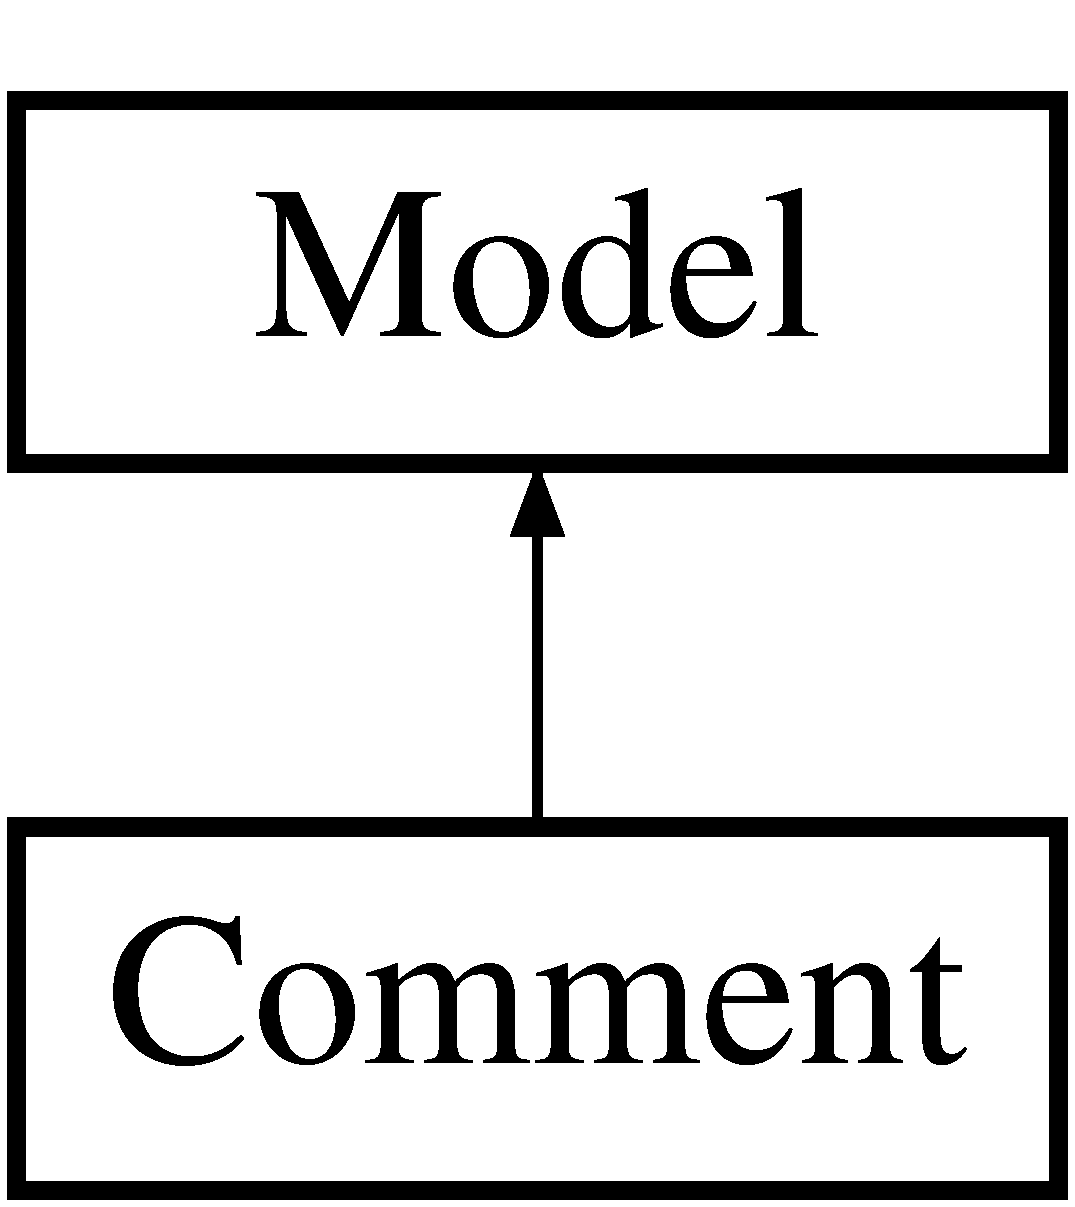
\includegraphics[height=2.000000cm]{classapp_1_1models_1_1_comment}
\end{center}
\end{figure}
\subsection*{Public Member Functions}
\begin{DoxyCompactItemize}
\item 
\hypertarget{classapp_1_1models_1_1_comment_a17dba92d96b9dd48c62f3ede3eef94d4}{}\label{classapp_1_1models_1_1_comment_a17dba92d96b9dd48c62f3ede3eef94d4} 
{\bfseries rules} ()
\item 
\hypertarget{classapp_1_1models_1_1_comment_a45fa8ff74582dbb9c4f54d46694f01db}{}\label{classapp_1_1models_1_1_comment_a45fa8ff74582dbb9c4f54d46694f01db} 
{\bfseries add\+Comment} (\$order\+Id, \$user\+Id)
\item 
\hypertarget{classapp_1_1models_1_1_comment_a7b020e66baff292f121ae507294a84b1}{}\label{classapp_1_1models_1_1_comment_a7b020e66baff292f121ae507294a84b1} 
{\bfseries calc\+Rating} (\$user\+Id, \$flag)
\item 
\hypertarget{classapp_1_1models_1_1_comment_a09847fa3ea7e3ef93e703be2ea161d45}{}\label{classapp_1_1models_1_1_comment_a09847fa3ea7e3ef93e703be2ea161d45} 
{\bfseries get\+User\+Empl\+Comments} (\$user\+Id)
\item 
\hypertarget{classapp_1_1models_1_1_comment_a9b3a5dacb33575cdc4ec086ffc88f9aa}{}\label{classapp_1_1models_1_1_comment_a9b3a5dacb33575cdc4ec086ffc88f9aa} 
{\bfseries get\+User\+Cust\+Comments} (\$user\+Id)
\item 
\hypertarget{classapp_1_1models_1_1_comment_ad75c16015a54db10075453d0ab31aa71}{}\label{classapp_1_1models_1_1_comment_ad75c16015a54db10075453d0ab31aa71} 
{\bfseries get\+Send\+Empl\+Comments} (\$user\+Id)
\item 
\hypertarget{classapp_1_1models_1_1_comment_acbbb2a29fac4fc3870d5d84c495de3f7}{}\label{classapp_1_1models_1_1_comment_acbbb2a29fac4fc3870d5d84c495de3f7} 
{\bfseries edit\+Comment} (\$id)
\item 
\hypertarget{classapp_1_1models_1_1_comment_ac8e85a14c66da26256047c07602ae38f}{}\label{classapp_1_1models_1_1_comment_ac8e85a14c66da26256047c07602ae38f} 
{\bfseries get\+Send\+Cust\+Comment} (\$user\+Id)
\end{DoxyCompactItemize}
\subsection*{Static Public Member Functions}
\begin{DoxyCompactItemize}
\item 
\hypertarget{classapp_1_1models_1_1_comment_a44672f6fe5c05d1a152e44b3843365ce}{}\label{classapp_1_1models_1_1_comment_a44672f6fe5c05d1a152e44b3843365ce} 
static {\bfseries has\+User\+Comment} (\$order\+Id, \$user\+Id=null)
\end{DoxyCompactItemize}
\subsection*{Data Fields}
\begin{DoxyCompactItemize}
\item 
\hypertarget{classapp_1_1models_1_1_comment_ae97941710d863131c700f069b109991e}{}\label{classapp_1_1models_1_1_comment_ae97941710d863131c700f069b109991e} 
{\bfseries \$id}
\item 
\hypertarget{classapp_1_1models_1_1_comment_ad0834b3f78c37216b0ba8d6b598364b2}{}\label{classapp_1_1models_1_1_comment_ad0834b3f78c37216b0ba8d6b598364b2} 
{\bfseries \$creator\+Id}
\item 
\hypertarget{classapp_1_1models_1_1_comment_adf95f30eaafccead90ab5e2cdb55e9b9}{}\label{classapp_1_1models_1_1_comment_adf95f30eaafccead90ab5e2cdb55e9b9} 
{\bfseries \$text}
\item 
\hypertarget{classapp_1_1models_1_1_comment_a01cea456eabd700254653d5b8dcaba9d}{}\label{classapp_1_1models_1_1_comment_a01cea456eabd700254653d5b8dcaba9d} 
{\bfseries \$time\+Posted}
\item 
\hypertarget{classapp_1_1models_1_1_comment_a44118acf7e954a3bc096a4af6b059c23}{}\label{classapp_1_1models_1_1_comment_a44118acf7e954a3bc096a4af6b059c23} 
{\bfseries \$rating}
\end{DoxyCompactItemize}


The documentation for this class was generated from the following file\+:\begin{DoxyCompactItemize}
\item 
Comment.\+php\end{DoxyCompactItemize}

\hypertarget{classapp_1_1models_1_1_comments}{}\section{Comments Class Reference}
\label{classapp_1_1models_1_1_comments}\index{Comments@{Comments}}
Inheritance diagram for Comments\+:\begin{figure}[H]
\begin{center}
\leavevmode
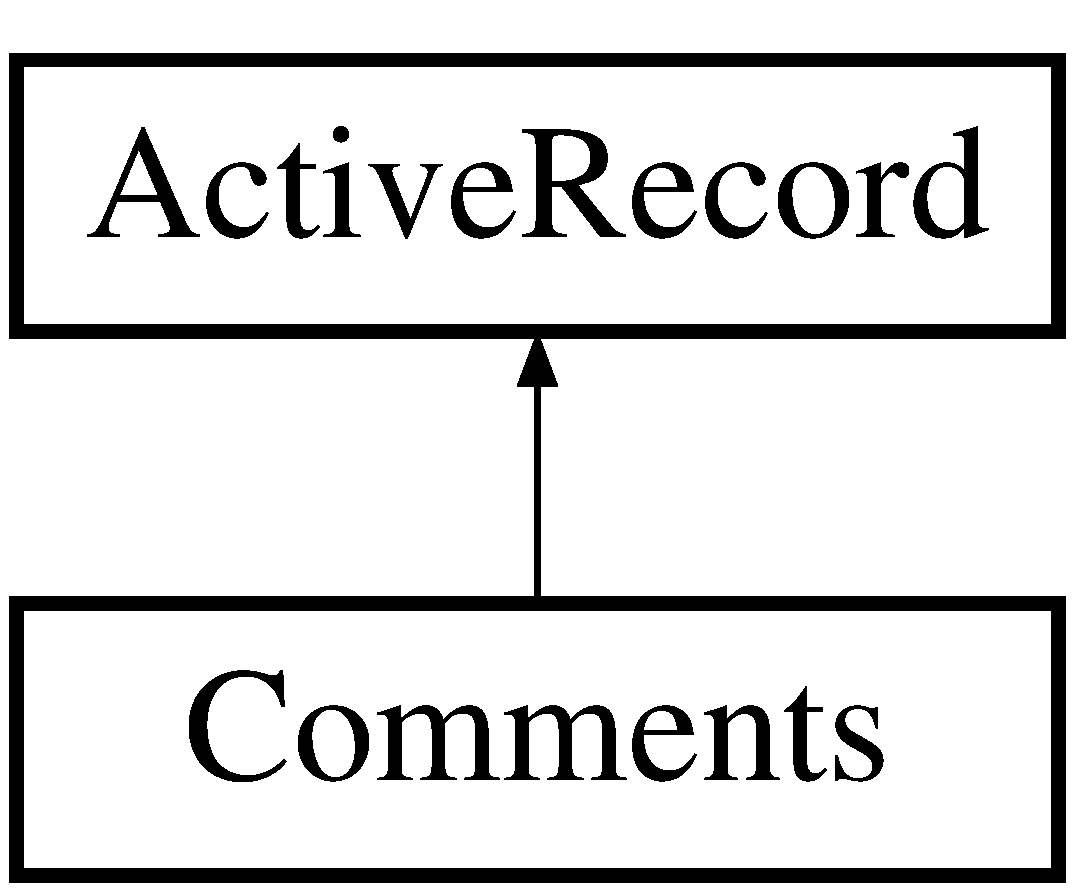
\includegraphics[height=2.000000cm]{classapp_1_1models_1_1_comments}
\end{center}
\end{figure}
\subsection*{Public Member Functions}
\begin{DoxyCompactItemize}
\item 
\hypertarget{classapp_1_1models_1_1_comments_a0f3e89d558c0892aebe1c8d8bb688064}{}\label{classapp_1_1models_1_1_comments_a0f3e89d558c0892aebe1c8d8bb688064} 
{\bfseries get\+Creator\+User} ()
\item 
\hypertarget{classapp_1_1models_1_1_comments_a52f1787c1a4941f65bf728ff3289b626}{}\label{classapp_1_1models_1_1_comments_a52f1787c1a4941f65bf728ff3289b626} 
{\bfseries get\+Order} ()
\end{DoxyCompactItemize}


The documentation for this class was generated from the following file\+:\begin{DoxyCompactItemize}
\item 
Comments.\+php\end{DoxyCompactItemize}

\hypertarget{classapp_1_1models_1_1_delivery_orders}{}\section{Delivery\+Orders Class Reference}
\label{classapp_1_1models_1_1_delivery_orders}\index{Delivery\+Orders@{Delivery\+Orders}}
Inheritance diagram for Delivery\+Orders\+:\begin{figure}[H]
\begin{center}
\leavevmode
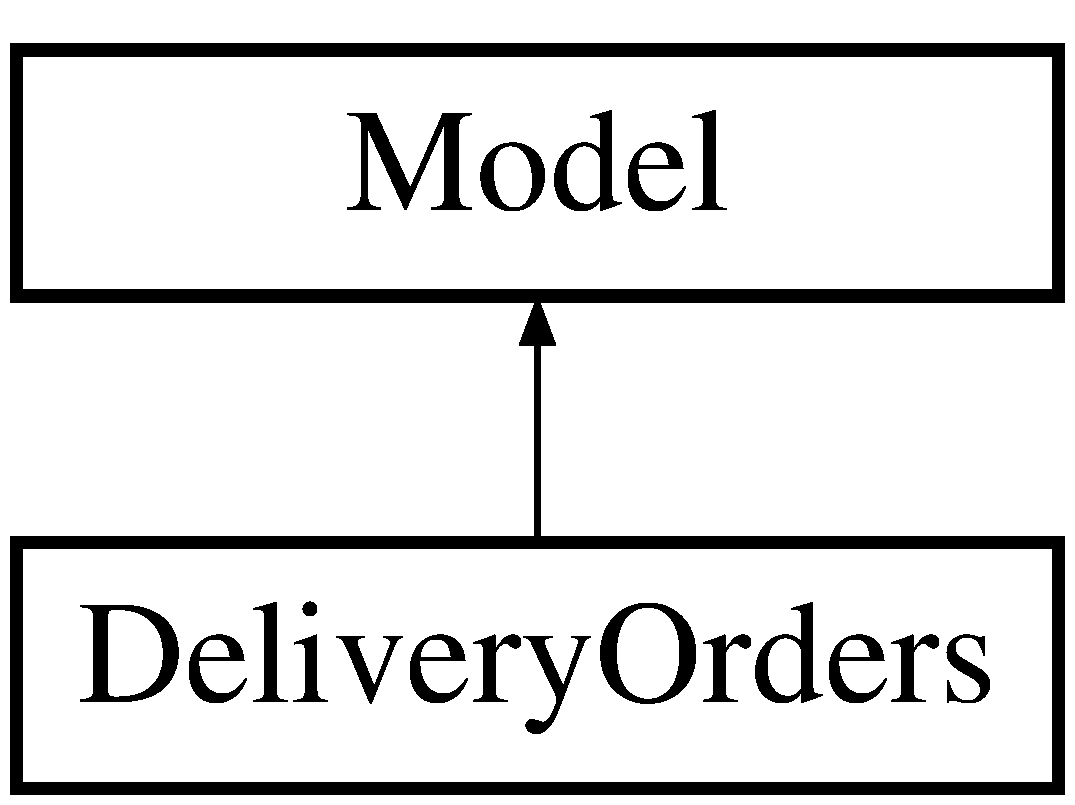
\includegraphics[height=2.000000cm]{classapp_1_1models_1_1_delivery_orders}
\end{center}
\end{figure}
\subsection*{Public Member Functions}
\begin{DoxyCompactItemize}
\item 
\hypertarget{classapp_1_1models_1_1_delivery_orders_a17dba92d96b9dd48c62f3ede3eef94d4}{}\label{classapp_1_1models_1_1_delivery_orders_a17dba92d96b9dd48c62f3ede3eef94d4} 
{\bfseries rules} ()
\item 
\hypertarget{classapp_1_1models_1_1_delivery_orders_a260288621b9c0c6f06b646f529721221}{}\label{classapp_1_1models_1_1_delivery_orders_a260288621b9c0c6f06b646f529721221} 
{\bfseries get\+Orders} (\$sort\+Method=null, \$date, \$time, \$price, \$search)
\item 
\hypertarget{classapp_1_1models_1_1_delivery_orders_a086cbd3798a8cf6d830dad6fb1612e63}{}\label{classapp_1_1models_1_1_delivery_orders_a086cbd3798a8cf6d830dad6fb1612e63} 
{\bfseries get\+User\+Orders} ()
\item 
\hypertarget{classapp_1_1models_1_1_delivery_orders_a08bac5dcb5e3342f2579685e1e992422}{}\label{classapp_1_1models_1_1_delivery_orders_a08bac5dcb5e3342f2579685e1e992422} 
{\bfseries get\+History\+Orders} ()
\item 
\hypertarget{classapp_1_1models_1_1_delivery_orders_a349504334b35d0f70ad125f6f8f6f2c4}{}\label{classapp_1_1models_1_1_delivery_orders_a349504334b35d0f70ad125f6f8f6f2c4} 
{\bfseries get\+User\+History\+Orders} ()
\item 
\hypertarget{classapp_1_1models_1_1_delivery_orders_a09c9cfa97d9cd97e55847fed54bbef96}{}\label{classapp_1_1models_1_1_delivery_orders_a09c9cfa97d9cd97e55847fed54bbef96} 
{\bfseries get\+User\+Requests\+Id} (\$status=null)
\item 
\hypertarget{classapp_1_1models_1_1_delivery_orders_a392acdf11aef3ebdb6d394e5f97d1dab}{}\label{classapp_1_1models_1_1_delivery_orders_a392acdf11aef3ebdb6d394e5f97d1dab} 
{\bfseries get\+User\+Orders\+In\+Process} (\$user\+Id)
\item 
\hypertarget{classapp_1_1models_1_1_delivery_orders_a7a254a52dadfcb4672de8791c6b0d5e8}{}\label{classapp_1_1models_1_1_delivery_orders_a7a254a52dadfcb4672de8791c6b0d5e8} 
{\bfseries get\+User\+Requests} ()
\item 
\hypertarget{classapp_1_1models_1_1_delivery_orders_ac1aeb6ab950d820bdaa381b8e58c0af4}{}\label{classapp_1_1models_1_1_delivery_orders_ac1aeb6ab950d820bdaa381b8e58c0af4} 
{\bfseries orders\+Count} ()
\end{DoxyCompactItemize}
\subsection*{Data Fields}
\begin{DoxyCompactItemize}
\item 
\hypertarget{classapp_1_1models_1_1_delivery_orders_a481c918f8d853749e00b5942cabf599a}{}\label{classapp_1_1models_1_1_delivery_orders_a481c918f8d853749e00b5942cabf599a} 
{\bfseries \$date}
\item 
\hypertarget{classapp_1_1models_1_1_delivery_orders_a9ece7043091b6a51af5679649e67b7cd}{}\label{classapp_1_1models_1_1_delivery_orders_a9ece7043091b6a51af5679649e67b7cd} 
{\bfseries \$time\+Start}
\item 
\hypertarget{classapp_1_1models_1_1_delivery_orders_a881c9cd0de6e69171af6cdfeb108da0c}{}\label{classapp_1_1models_1_1_delivery_orders_a881c9cd0de6e69171af6cdfeb108da0c} 
{\bfseries \$time\+End}
\item 
\hypertarget{classapp_1_1models_1_1_delivery_orders_a3a29daa6c3b624c09ed790e3228ed67e}{}\label{classapp_1_1models_1_1_delivery_orders_a3a29daa6c3b624c09ed790e3228ed67e} 
{\bfseries \$min\+Price}
\item 
\hypertarget{classapp_1_1models_1_1_delivery_orders_aec4de82415d7f05cb9748d12d3a95a87}{}\label{classapp_1_1models_1_1_delivery_orders_aec4de82415d7f05cb9748d12d3a95a87} 
{\bfseries \$offset}
\end{DoxyCompactItemize}


The documentation for this class was generated from the following file\+:\begin{DoxyCompactItemize}
\item 
Delivery\+Orders.\+php\end{DoxyCompactItemize}

\hypertarget{classapp_1_1models_1_1_entry_form}{}\section{Entry\+Form Class Reference}
\label{classapp_1_1models_1_1_entry_form}\index{Entry\+Form@{Entry\+Form}}
Inheritance diagram for Entry\+Form\+:\begin{figure}[H]
\begin{center}
\leavevmode
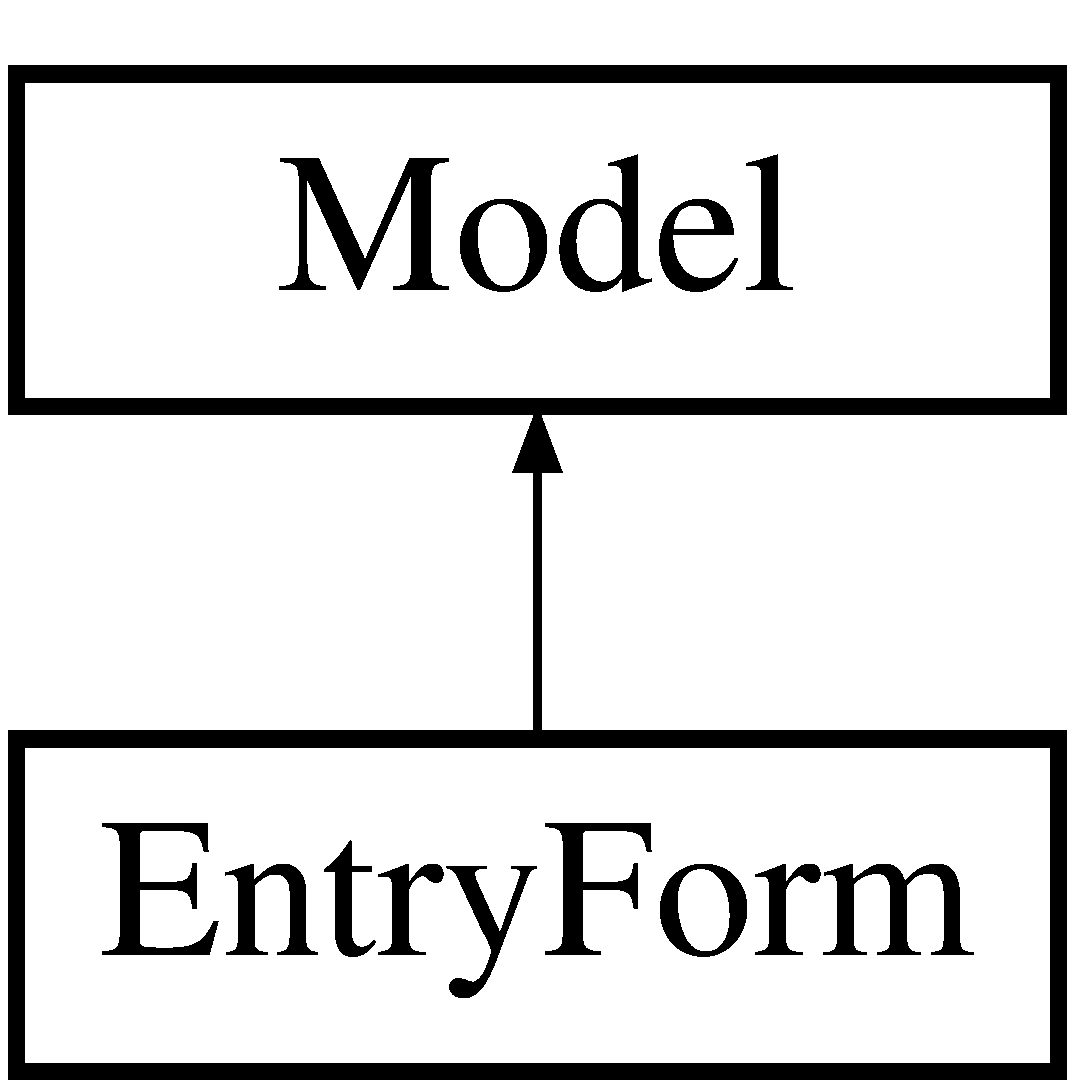
\includegraphics[height=2.000000cm]{classapp_1_1models_1_1_entry_form}
\end{center}
\end{figure}
\subsection*{Public Member Functions}
\begin{DoxyCompactItemize}
\item 
\hypertarget{classapp_1_1models_1_1_entry_form_a17dba92d96b9dd48c62f3ede3eef94d4}{}\label{classapp_1_1models_1_1_entry_form_a17dba92d96b9dd48c62f3ede3eef94d4} 
{\bfseries rules} ()
\end{DoxyCompactItemize}
\subsection*{Data Fields}
\begin{DoxyCompactItemize}
\item 
\hypertarget{classapp_1_1models_1_1_entry_form_ab2fc40d43824ea3e1ce5d86dee0d763b}{}\label{classapp_1_1models_1_1_entry_form_ab2fc40d43824ea3e1ce5d86dee0d763b} 
{\bfseries \$name}
\item 
\hypertarget{classapp_1_1models_1_1_entry_form_ad634f418b20382e2802f80532d76d3cd}{}\label{classapp_1_1models_1_1_entry_form_ad634f418b20382e2802f80532d76d3cd} 
{\bfseries \$email}
\end{DoxyCompactItemize}


The documentation for this class was generated from the following file\+:\begin{DoxyCompactItemize}
\item 
Entry\+Form.\+php\end{DoxyCompactItemize}

\hypertarget{classapp_1_1models_1_1_items}{}\section{Items Class Reference}
\label{classapp_1_1models_1_1_items}\index{Items@{Items}}
Inheritance diagram for Items\+:\begin{figure}[H]
\begin{center}
\leavevmode
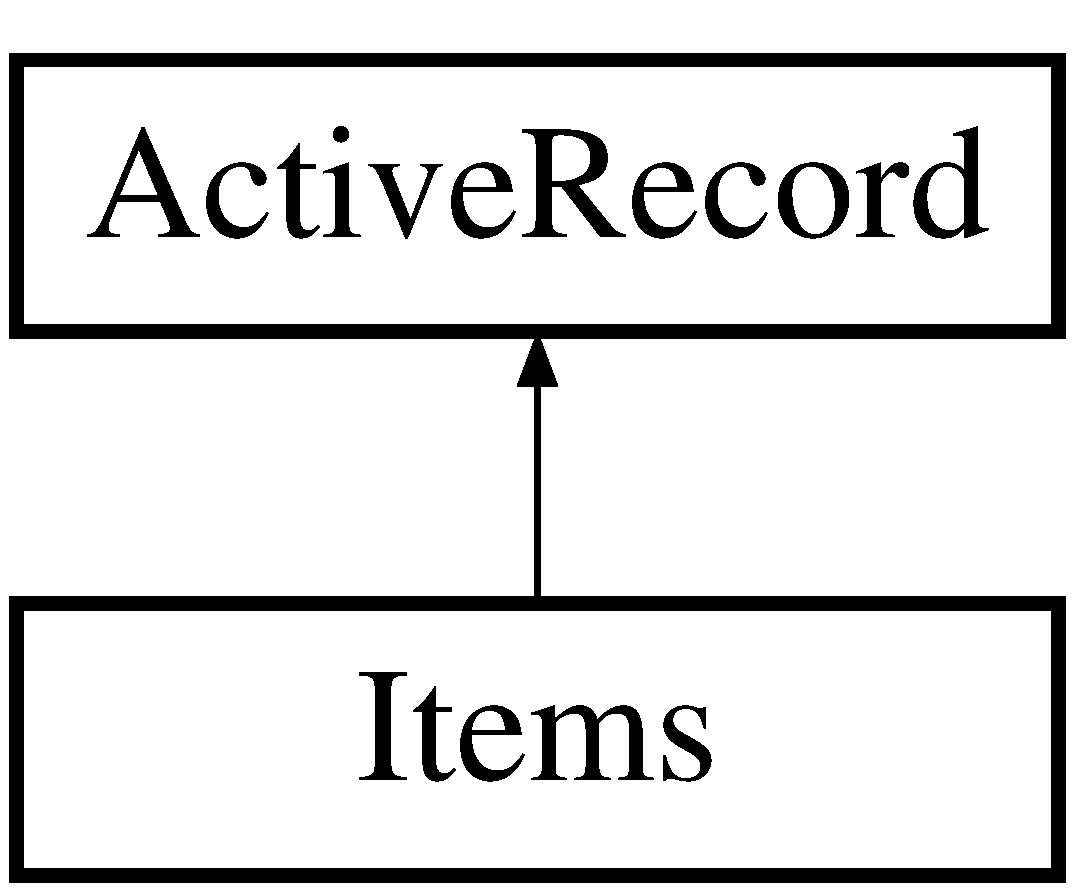
\includegraphics[height=2.000000cm]{classapp_1_1models_1_1_items}
\end{center}
\end{figure}


The documentation for this class was generated from the following file\+:\begin{DoxyCompactItemize}
\item 
Items.\+php\end{DoxyCompactItemize}

\hypertarget{classapp_1_1models_1_1_login_form}{}\section{Login\+Form Class Reference}
\label{classapp_1_1models_1_1_login_form}\index{Login\+Form@{Login\+Form}}
Inheritance diagram for Login\+Form\+:\begin{figure}[H]
\begin{center}
\leavevmode
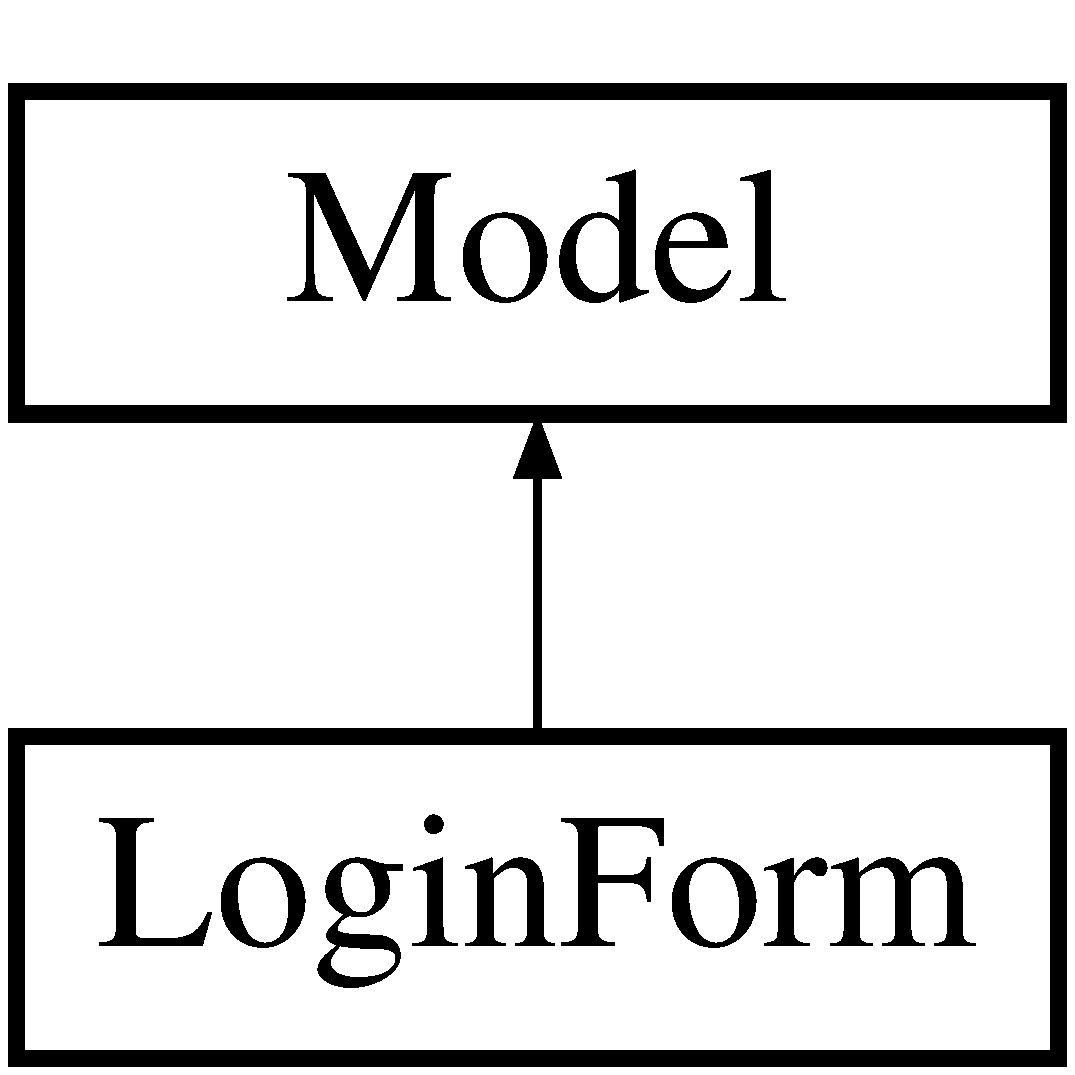
\includegraphics[height=2.000000cm]{classapp_1_1models_1_1_login_form}
\end{center}
\end{figure}
\subsection*{Public Member Functions}
\begin{DoxyCompactItemize}
\item 
\hyperlink{classapp_1_1models_1_1_login_form_a17dba92d96b9dd48c62f3ede3eef94d4}{rules} ()
\item 
\hyperlink{classapp_1_1models_1_1_login_form_aa188862aeb325bc1c2be6d8d89893787}{validate\+Password} (\$attribute, \$params)
\item 
\hyperlink{classapp_1_1models_1_1_login_form_aa311da27ba5706f5710cea7706c8eae1}{login} ()
\item 
\hyperlink{classapp_1_1models_1_1_login_form_ae81b7186fb97a7c6457edcc68c9aa2ef}{get\+User} ()
\end{DoxyCompactItemize}
\subsection*{Data Fields}
\begin{DoxyCompactItemize}
\item 
\hypertarget{classapp_1_1models_1_1_login_form_a0eb82aa5f81cf845de4b36cd653c42cf}{}\label{classapp_1_1models_1_1_login_form_a0eb82aa5f81cf845de4b36cd653c42cf} 
{\bfseries \$username}
\item 
\hypertarget{classapp_1_1models_1_1_login_form_a607686ef9f99ea7c42f4f3dd3dbb2b0d}{}\label{classapp_1_1models_1_1_login_form_a607686ef9f99ea7c42f4f3dd3dbb2b0d} 
{\bfseries \$password}
\item 
\hypertarget{classapp_1_1models_1_1_login_form_ad9e6993ef3c93c464ec55f7d7e5d1ac9}{}\label{classapp_1_1models_1_1_login_form_ad9e6993ef3c93c464ec55f7d7e5d1ac9} 
{\bfseries \$remember\+Me} = true
\end{DoxyCompactItemize}


\subsection{Member Function Documentation}
\hypertarget{classapp_1_1models_1_1_login_form_ae81b7186fb97a7c6457edcc68c9aa2ef}{}\label{classapp_1_1models_1_1_login_form_ae81b7186fb97a7c6457edcc68c9aa2ef} 
\index{app\+::models\+::\+Login\+Form@{app\+::models\+::\+Login\+Form}!get\+User@{get\+User}}
\index{get\+User@{get\+User}!app\+::models\+::\+Login\+Form@{app\+::models\+::\+Login\+Form}}
\subsubsection{\texorpdfstring{get\+User()}{getUser()}}
{\footnotesize\ttfamily get\+User (\begin{DoxyParamCaption}{ }\end{DoxyParamCaption})}

Finds user by \mbox{[}\mbox{[}username\mbox{]}\mbox{]}

\begin{DoxyReturn}{Returns}
User$\vert$null 
\end{DoxyReturn}
\hypertarget{classapp_1_1models_1_1_login_form_aa311da27ba5706f5710cea7706c8eae1}{}\label{classapp_1_1models_1_1_login_form_aa311da27ba5706f5710cea7706c8eae1} 
\index{app\+::models\+::\+Login\+Form@{app\+::models\+::\+Login\+Form}!login@{login}}
\index{login@{login}!app\+::models\+::\+Login\+Form@{app\+::models\+::\+Login\+Form}}
\subsubsection{\texorpdfstring{login()}{login()}}
{\footnotesize\ttfamily login (\begin{DoxyParamCaption}{ }\end{DoxyParamCaption})}

Logs in a user using the provided username and password. \begin{DoxyReturn}{Returns}
boolean whether the user is logged in successfully 
\end{DoxyReturn}
\hypertarget{classapp_1_1models_1_1_login_form_a17dba92d96b9dd48c62f3ede3eef94d4}{}\label{classapp_1_1models_1_1_login_form_a17dba92d96b9dd48c62f3ede3eef94d4} 
\index{app\+::models\+::\+Login\+Form@{app\+::models\+::\+Login\+Form}!rules@{rules}}
\index{rules@{rules}!app\+::models\+::\+Login\+Form@{app\+::models\+::\+Login\+Form}}
\subsubsection{\texorpdfstring{rules()}{rules()}}
{\footnotesize\ttfamily rules (\begin{DoxyParamCaption}{ }\end{DoxyParamCaption})}

\begin{DoxyReturn}{Returns}
array the validation rules. 
\end{DoxyReturn}
\hypertarget{classapp_1_1models_1_1_login_form_aa188862aeb325bc1c2be6d8d89893787}{}\label{classapp_1_1models_1_1_login_form_aa188862aeb325bc1c2be6d8d89893787} 
\index{app\+::models\+::\+Login\+Form@{app\+::models\+::\+Login\+Form}!validate\+Password@{validate\+Password}}
\index{validate\+Password@{validate\+Password}!app\+::models\+::\+Login\+Form@{app\+::models\+::\+Login\+Form}}
\subsubsection{\texorpdfstring{validate\+Password()}{validatePassword()}}
{\footnotesize\ttfamily validate\+Password (\begin{DoxyParamCaption}\item[{}]{\$attribute,  }\item[{}]{\$params }\end{DoxyParamCaption})}

Validates the password. This method serves as the inline validation for password.


\begin{DoxyParams}[1]{Parameters}
string & {\em \$attribute} & the attribute currently being validated \\
\hline
array & {\em \$params} & the additional name-\/value pairs given in the rule \\
\hline
\end{DoxyParams}


The documentation for this class was generated from the following file\+:\begin{DoxyCompactItemize}
\item 
Login\+Form.\+php\end{DoxyCompactItemize}

\hypertarget{classapp_1_1models_1_1_order}{}\section{Order Class Reference}
\label{classapp_1_1models_1_1_order}\index{Order@{Order}}
Inheritance diagram for Order\+:\begin{figure}[H]
\begin{center}
\leavevmode
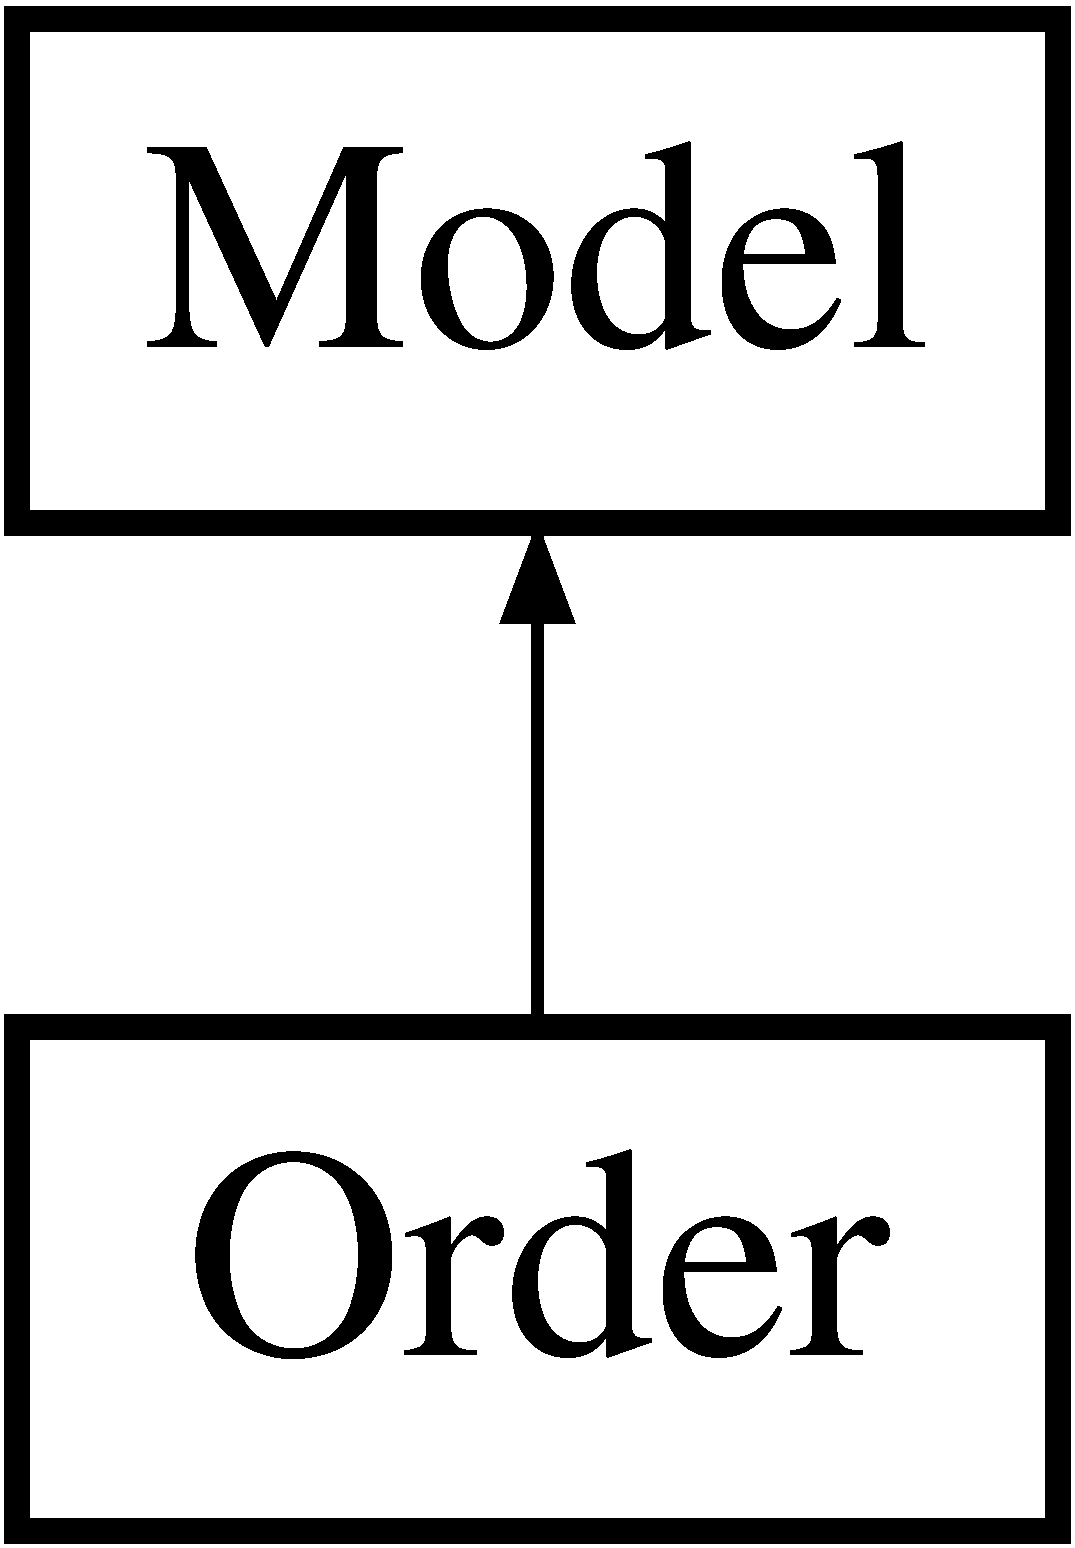
\includegraphics[height=2.000000cm]{classapp_1_1models_1_1_order}
\end{center}
\end{figure}
\subsection*{Public Member Functions}
\begin{DoxyCompactItemize}
\item 
\hypertarget{classapp_1_1models_1_1_order_a17dba92d96b9dd48c62f3ede3eef94d4}{}\label{classapp_1_1models_1_1_order_a17dba92d96b9dd48c62f3ede3eef94d4} 
{\bfseries rules} ()
\item 
\hypertarget{classapp_1_1models_1_1_order_afd2e4b9f8bf18ff12e1c13c06fd0438d}{}\label{classapp_1_1models_1_1_order_afd2e4b9f8bf18ff12e1c13c06fd0438d} 
{\bfseries form\+Name} ()
\item 
\hypertarget{classapp_1_1models_1_1_order_a3ee5031f29f0a213e6e9aaeb6b1cbaf6}{}\label{classapp_1_1models_1_1_order_a3ee5031f29f0a213e6e9aaeb6b1cbaf6} 
{\bfseries add\+Order} ()
\item 
\hypertarget{classapp_1_1models_1_1_order_ac3a4371fdbba188b1545a8e77d222bb1}{}\label{classapp_1_1models_1_1_order_ac3a4371fdbba188b1545a8e77d222bb1} 
{\bfseries add\+Items} (\$items)
\item 
\hypertarget{classapp_1_1models_1_1_order_a41667b506246cdab68dfde8bf6bf9f73}{}\label{classapp_1_1models_1_1_order_a41667b506246cdab68dfde8bf6bf9f73} 
{\bfseries get\+Items\+By\+Order\+Id} (\$id)
\item 
\hypertarget{classapp_1_1models_1_1_order_a7cd29143d80b25263fca798fbca75474}{}\label{classapp_1_1models_1_1_order_a7cd29143d80b25263fca798fbca75474} 
{\bfseries delete\+Order\+By\+Id} (\$id)
\item 
\hypertarget{classapp_1_1models_1_1_order_a17b0e0eec2ecf37ae07fd0e7743db245}{}\label{classapp_1_1models_1_1_order_a17b0e0eec2ecf37ae07fd0e7743db245} 
{\bfseries edit\+Order} (\$id)
\item 
\hypertarget{classapp_1_1models_1_1_order_ab20ac3660e2d867b235b004bd3950ec3}{}\label{classapp_1_1models_1_1_order_ab20ac3660e2d867b235b004bd3950ec3} 
{\bfseries get\+Items} ()
\item 
\hypertarget{classapp_1_1models_1_1_order_aa7b4f361a03c18924cf724c49647a525}{}\label{classapp_1_1models_1_1_order_aa7b4f361a03c18924cf724c49647a525} 
{\bfseries get\+Creator\+Login} ()
\item 
\hypertarget{classapp_1_1models_1_1_order_a3346e13f18c329be8e4754296e5e2f04}{}\label{classapp_1_1models_1_1_order_a3346e13f18c329be8e4754296e5e2f04} 
{\bfseries generate\+Date} (\$flag)
\item 
\hypertarget{classapp_1_1models_1_1_order_a6c016fc42dc005b154ec760484838d6f}{}\label{classapp_1_1models_1_1_order_a6c016fc42dc005b154ec760484838d6f} 
{\bfseries get\+User\+City} ()
\item 
\hypertarget{classapp_1_1models_1_1_order_ae835fb16cefe7ee68a0c422c5b0d475c}{}\label{classapp_1_1models_1_1_order_ae835fb16cefe7ee68a0c422c5b0d475c} 
{\bfseries get\+Time\+Posted} ()
\end{DoxyCompactItemize}
\subsection*{Static Public Member Functions}
\begin{DoxyCompactItemize}
\item 
\hypertarget{classapp_1_1models_1_1_order_abc825d65e740b81ed3dda6d3ad62760d}{}\label{classapp_1_1models_1_1_order_abc825d65e740b81ed3dda6d3ad62760d} 
static {\bfseries get\+Order\+By\+Id} (\$id)
\item 
\hypertarget{classapp_1_1models_1_1_order_a783e0463c7c27ee9b15b1e3bc345550d}{}\label{classapp_1_1models_1_1_order_a783e0463c7c27ee9b15b1e3bc345550d} 
static {\bfseries is\+Users\+Order} (\$id)
\item 
\hypertarget{classapp_1_1models_1_1_order_abbea95ee2b9586ebf32787e9807a9a0a}{}\label{classapp_1_1models_1_1_order_abbea95ee2b9586ebf32787e9807a9a0a} 
static {\bfseries is\+User\+Executor} (\$user\+Id, \$order\+Id)
\item 
\hypertarget{classapp_1_1models_1_1_order_a0b89352bd73b940331e04c65a13167a9}{}\label{classapp_1_1models_1_1_order_a0b89352bd73b940331e04c65a13167a9} 
static {\bfseries is\+Order\+In\+Process} (\$id)
\item 
\hypertarget{classapp_1_1models_1_1_order_ad123b6765ef4118ff6f4c2840a6f634d}{}\label{classapp_1_1models_1_1_order_ad123b6765ef4118ff6f4c2840a6f634d} 
static {\bfseries count\+Empl\+User\+Orders} (\$id)
\item 
\hypertarget{classapp_1_1models_1_1_order_a82f98573ef4d48854a42bceb54e83815}{}\label{classapp_1_1models_1_1_order_a82f98573ef4d48854a42bceb54e83815} 
static {\bfseries count\+User\+Done\+Orders} (\$id)
\end{DoxyCompactItemize}
\subsection*{Data Fields}
\begin{DoxyCompactItemize}
\item 
\hypertarget{classapp_1_1models_1_1_order_ae97941710d863131c700f069b109991e}{}\label{classapp_1_1models_1_1_order_ae97941710d863131c700f069b109991e} 
{\bfseries \$id}
\item 
\hypertarget{classapp_1_1models_1_1_order_ada57e7bb7c152edad18fe2f166188691}{}\label{classapp_1_1models_1_1_order_ada57e7bb7c152edad18fe2f166188691} 
{\bfseries \$title}
\item 
\hypertarget{classapp_1_1models_1_1_order_a51c1f7f25645a07747fa01f228379fec}{}\label{classapp_1_1models_1_1_order_a51c1f7f25645a07747fa01f228379fec} 
{\bfseries \$order\+Date}
\item 
\hypertarget{classapp_1_1models_1_1_order_a5333f745a6658b550580058a49045aa6}{}\label{classapp_1_1models_1_1_order_a5333f745a6658b550580058a49045aa6} 
{\bfseries \$time\+Min}
\item 
\hypertarget{classapp_1_1models_1_1_order_ab808cd870015a2884e59c4678f9a54c9}{}\label{classapp_1_1models_1_1_order_ab808cd870015a2884e59c4678f9a54c9} 
{\bfseries \$time\+Max}
\item 
\hypertarget{classapp_1_1models_1_1_order_a87b032cba06009e3467abf1c8018d960}{}\label{classapp_1_1models_1_1_order_a87b032cba06009e3467abf1c8018d960} 
{\bfseries \$description}
\item 
\hypertarget{classapp_1_1models_1_1_order_a264091074b1a8f4ed0abefd278831f6f}{}\label{classapp_1_1models_1_1_order_a264091074b1a8f4ed0abefd278831f6f} 
{\bfseries \$price}
\item 
\hypertarget{classapp_1_1models_1_1_order_ad9b483d997a82a0edafc4bde35623d1c}{}\label{classapp_1_1models_1_1_order_ad9b483d997a82a0edafc4bde35623d1c} 
{\bfseries \$start\+Hour}
\item 
\hypertarget{classapp_1_1models_1_1_order_af2e188a163893425afeca92f9e13b8f2}{}\label{classapp_1_1models_1_1_order_af2e188a163893425afeca92f9e13b8f2} 
{\bfseries \$end\+Hour}
\item 
\hypertarget{classapp_1_1models_1_1_order_a56867ee79b138bae27ff55326b67d014}{}\label{classapp_1_1models_1_1_order_a56867ee79b138bae27ff55326b67d014} 
{\bfseries \$start\+Minutes}
\item 
\hypertarget{classapp_1_1models_1_1_order_a0f7c9896d989d4c8261db201fadfe194}{}\label{classapp_1_1models_1_1_order_a0f7c9896d989d4c8261db201fadfe194} 
{\bfseries \$end\+Minutes}
\item 
\hypertarget{classapp_1_1models_1_1_order_a737abdef83dabb219182c1e88887c6c3}{}\label{classapp_1_1models_1_1_order_a737abdef83dabb219182c1e88887c6c3} 
{\bfseries \$items}
\item 
\hypertarget{classapp_1_1models_1_1_order_abd9e73ab30c6a3dec0abe89bd2b55240}{}\label{classapp_1_1models_1_1_order_abd9e73ab30c6a3dec0abe89bd2b55240} 
{\bfseries \$request\+Num}
\end{DoxyCompactItemize}


The documentation for this class was generated from the following file\+:\begin{DoxyCompactItemize}
\item 
Order.\+php\end{DoxyCompactItemize}

\hypertarget{classapp_1_1models_1_1_order__requests}{}\section{Order\+\_\+requests Class Reference}
\label{classapp_1_1models_1_1_order__requests}\index{Order\+\_\+requests@{Order\+\_\+requests}}
Inheritance diagram for Order\+\_\+requests\+:\begin{figure}[H]
\begin{center}
\leavevmode
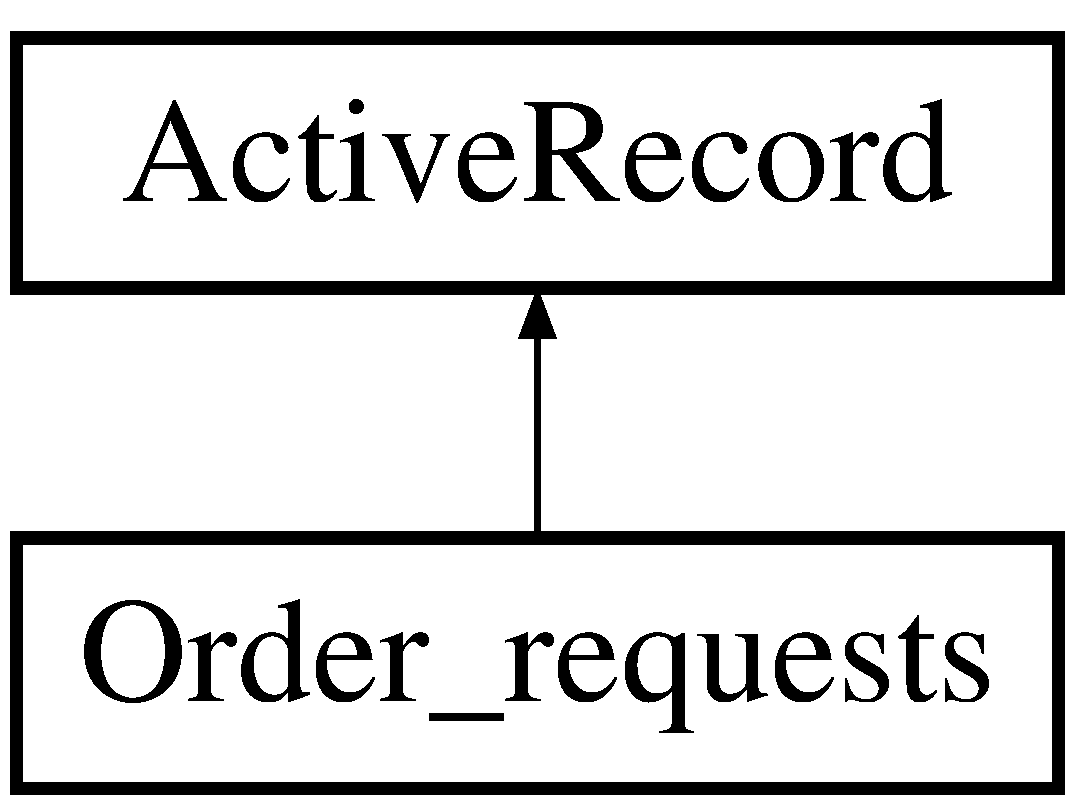
\includegraphics[height=2.000000cm]{classapp_1_1models_1_1_order__requests}
\end{center}
\end{figure}
\subsection*{Public Member Functions}
\begin{DoxyCompactItemize}
\item 
\hypertarget{classapp_1_1models_1_1_order__requests_a52f1787c1a4941f65bf728ff3289b626}{}\label{classapp_1_1models_1_1_order__requests_a52f1787c1a4941f65bf728ff3289b626} 
{\bfseries get\+Order} ()
\item 
\hypertarget{classapp_1_1models_1_1_order__requests_ae81b7186fb97a7c6457edcc68c9aa2ef}{}\label{classapp_1_1models_1_1_order__requests_ae81b7186fb97a7c6457edcc68c9aa2ef} 
{\bfseries get\+User} ()
\end{DoxyCompactItemize}


The documentation for this class was generated from the following file\+:\begin{DoxyCompactItemize}
\item 
Order\+\_\+requests.\+php\end{DoxyCompactItemize}

\hypertarget{classapp_1_1models_1_1_orders}{}\section{Orders Class Reference}
\label{classapp_1_1models_1_1_orders}\index{Orders@{Orders}}
Inheritance diagram for Orders\+:\begin{figure}[H]
\begin{center}
\leavevmode
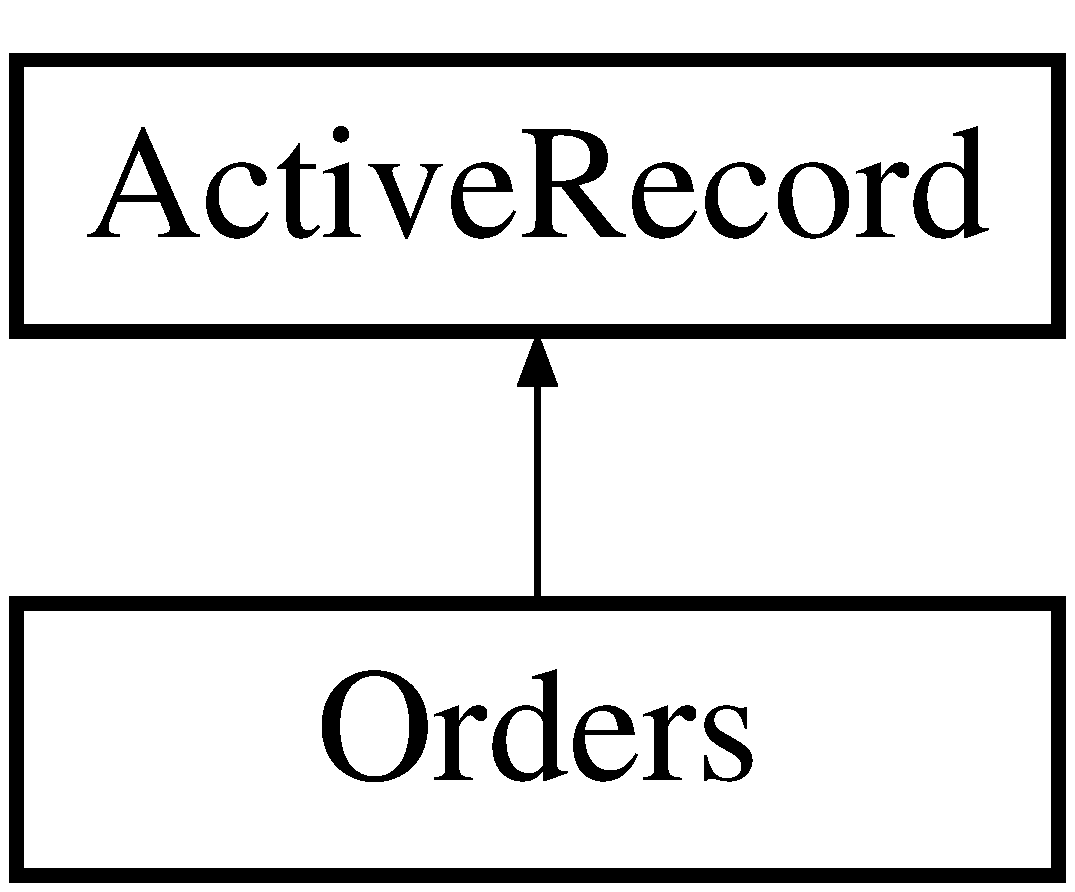
\includegraphics[height=2.000000cm]{classapp_1_1models_1_1_orders}
\end{center}
\end{figure}
\subsection*{Public Member Functions}
\begin{DoxyCompactItemize}
\item 
\hypertarget{classapp_1_1models_1_1_orders_a56ab3af6588561bfc165a1bb56983821}{}\label{classapp_1_1models_1_1_orders_a56ab3af6588561bfc165a1bb56983821} 
{\bfseries get\+Order\+\_\+requests} ()
\item 
\hypertarget{classapp_1_1models_1_1_orders_ae81b7186fb97a7c6457edcc68c9aa2ef}{}\label{classapp_1_1models_1_1_orders_ae81b7186fb97a7c6457edcc68c9aa2ef} 
{\bfseries get\+User} ()
\item 
\hypertarget{classapp_1_1models_1_1_orders_ab20ac3660e2d867b235b004bd3950ec3}{}\label{classapp_1_1models_1_1_orders_ab20ac3660e2d867b235b004bd3950ec3} 
{\bfseries get\+Items} ()
\item 
\hypertarget{classapp_1_1models_1_1_orders_a55b0fb55c00827c478acf035fd1a2ca0}{}\label{classapp_1_1models_1_1_orders_a55b0fb55c00827c478acf035fd1a2ca0} 
{\bfseries get\+Orders\+\_\+users} ()
\end{DoxyCompactItemize}


The documentation for this class was generated from the following file\+:\begin{DoxyCompactItemize}
\item 
Orders.\+php\end{DoxyCompactItemize}

\hypertarget{classapp_1_1models_1_1_orders__users}{}\section{Orders\+\_\+users Class Reference}
\label{classapp_1_1models_1_1_orders__users}\index{Orders\+\_\+users@{Orders\+\_\+users}}
Inheritance diagram for Orders\+\_\+users\+:\begin{figure}[H]
\begin{center}
\leavevmode
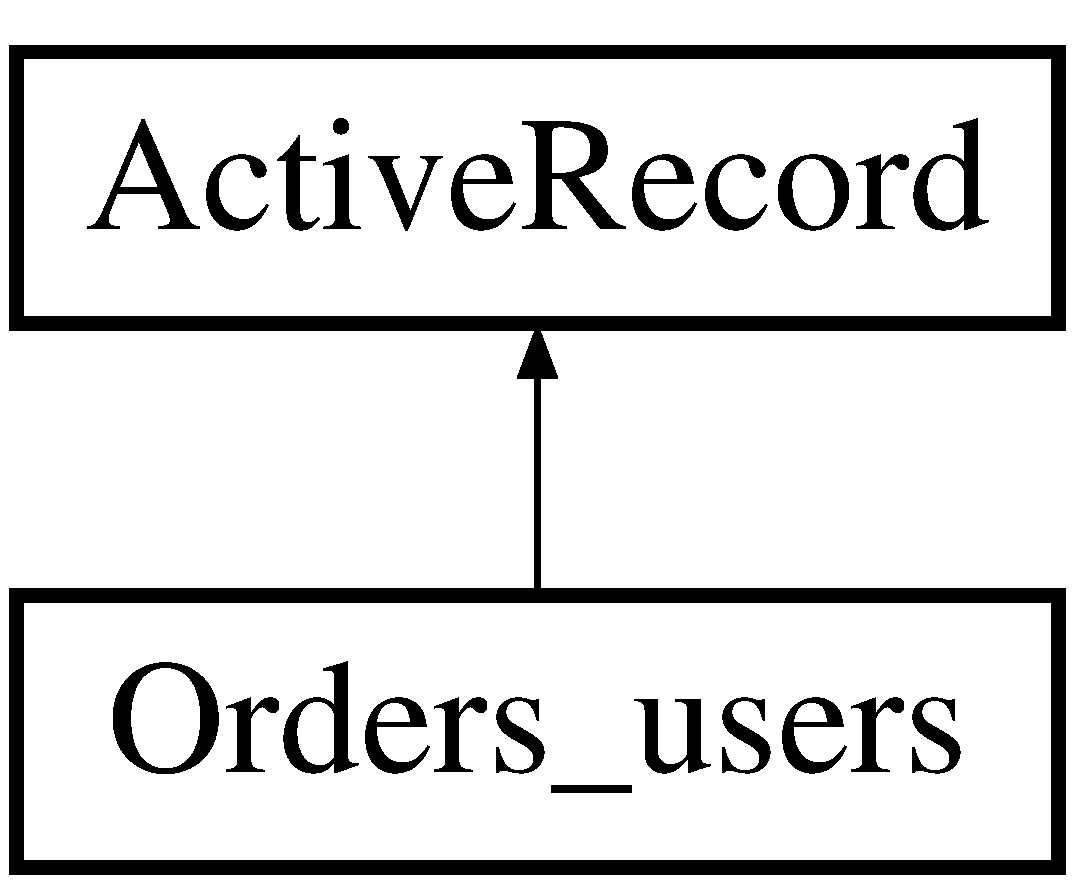
\includegraphics[height=2.000000cm]{classapp_1_1models_1_1_orders__users}
\end{center}
\end{figure}
\subsection*{Public Member Functions}
\begin{DoxyCompactItemize}
\item 
\hypertarget{classapp_1_1models_1_1_orders__users_ae81b7186fb97a7c6457edcc68c9aa2ef}{}\label{classapp_1_1models_1_1_orders__users_ae81b7186fb97a7c6457edcc68c9aa2ef} 
{\bfseries get\+User} ()
\item 
\hypertarget{classapp_1_1models_1_1_orders__users_a52f1787c1a4941f65bf728ff3289b626}{}\label{classapp_1_1models_1_1_orders__users_a52f1787c1a4941f65bf728ff3289b626} 
{\bfseries get\+Order} ()
\end{DoxyCompactItemize}


The documentation for this class was generated from the following file\+:\begin{DoxyCompactItemize}
\item 
Orders\+\_\+users.\+php\end{DoxyCompactItemize}

\hypertarget{classapp_1_1models_1_1_registration}{}\section{Registration Class Reference}
\label{classapp_1_1models_1_1_registration}\index{Registration@{Registration}}
Inheritance diagram for Registration\+:\begin{figure}[H]
\begin{center}
\leavevmode
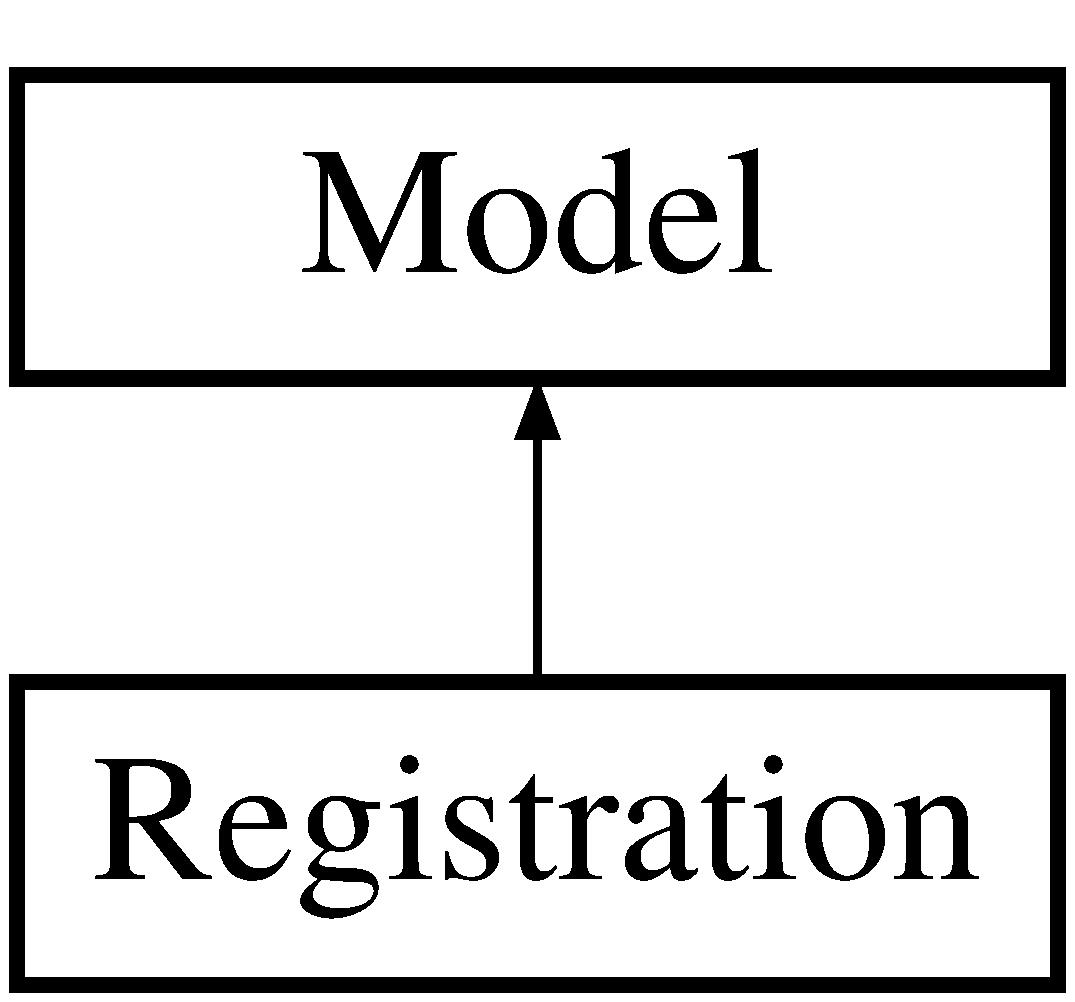
\includegraphics[height=2.000000cm]{classapp_1_1models_1_1_registration}
\end{center}
\end{figure}
\subsection*{Public Member Functions}
\begin{DoxyCompactItemize}
\item 
\hypertarget{classapp_1_1models_1_1_registration_a17dba92d96b9dd48c62f3ede3eef94d4}{}\label{classapp_1_1models_1_1_registration_a17dba92d96b9dd48c62f3ede3eef94d4} 
{\bfseries rules} ()
\item 
\hypertarget{classapp_1_1models_1_1_registration_a69ad61100b396854a498f1691c71bea6}{}\label{classapp_1_1models_1_1_registration_a69ad61100b396854a498f1691c71bea6} 
{\bfseries send\+Registration\+Email} ()
\item 
\hyperlink{classapp_1_1models_1_1_registration_a1fdb0f05b888f4aa92b319775e488e70}{register\+User} ()
\item 
\hypertarget{classapp_1_1models_1_1_registration_a7e2a269af301c25aa204dc5fd296ab89}{}\label{classapp_1_1models_1_1_registration_a7e2a269af301c25aa204dc5fd296ab89} 
{\bfseries registration\+Confirm} (\$reg\+Code)
\end{DoxyCompactItemize}
\subsection*{Data Fields}
\begin{DoxyCompactItemize}
\item 
\hypertarget{classapp_1_1models_1_1_registration_afc31993e855f9631572adfedcfe6f34b}{}\label{classapp_1_1models_1_1_registration_afc31993e855f9631572adfedcfe6f34b} 
{\bfseries \$login}
\item 
\hypertarget{classapp_1_1models_1_1_registration_a607686ef9f99ea7c42f4f3dd3dbb2b0d}{}\label{classapp_1_1models_1_1_registration_a607686ef9f99ea7c42f4f3dd3dbb2b0d} 
{\bfseries \$password}
\item 
\hypertarget{classapp_1_1models_1_1_registration_ad634f418b20382e2802f80532d76d3cd}{}\label{classapp_1_1models_1_1_registration_ad634f418b20382e2802f80532d76d3cd} 
{\bfseries \$email}
\item 
\hypertarget{classapp_1_1models_1_1_registration_ab2fc40d43824ea3e1ce5d86dee0d763b}{}\label{classapp_1_1models_1_1_registration_ab2fc40d43824ea3e1ce5d86dee0d763b} 
{\bfseries \$name}
\item 
\hypertarget{classapp_1_1models_1_1_registration_a1d2ddb6354180329b59e8b90ed94dc7f}{}\label{classapp_1_1models_1_1_registration_a1d2ddb6354180329b59e8b90ed94dc7f} 
{\bfseries \$lastname}
\item 
\hypertarget{classapp_1_1models_1_1_registration_a41cf1f5996c1bf764eca3ccffea485e4}{}\label{classapp_1_1models_1_1_registration_a41cf1f5996c1bf764eca3ccffea485e4} 
{\bfseries \$birthday}
\item 
\hypertarget{classapp_1_1models_1_1_registration_a87b032cba06009e3467abf1c8018d960}{}\label{classapp_1_1models_1_1_registration_a87b032cba06009e3467abf1c8018d960} 
{\bfseries \$description}
\end{DoxyCompactItemize}


\subsection{Member Function Documentation}
\hypertarget{classapp_1_1models_1_1_registration_a1fdb0f05b888f4aa92b319775e488e70}{}\label{classapp_1_1models_1_1_registration_a1fdb0f05b888f4aa92b319775e488e70} 
\index{app\+::models\+::\+Registration@{app\+::models\+::\+Registration}!register\+User@{register\+User}}
\index{register\+User@{register\+User}!app\+::models\+::\+Registration@{app\+::models\+::\+Registration}}
\subsubsection{\texorpdfstring{register\+User()}{registerUser()}}
{\footnotesize\ttfamily register\+User (\begin{DoxyParamCaption}{ }\end{DoxyParamCaption})}

Registrion new user. This method serves as user registration with confirm mailer.

\begin{DoxyReturn}{Returns}
boolean whether the registration form was validated successuly and mail was send. 
\end{DoxyReturn}


The documentation for this class was generated from the following file\+:\begin{DoxyCompactItemize}
\item 
Registration.\+php\end{DoxyCompactItemize}

\hypertarget{classapp_1_1models_1_1_request}{}\section{Request Class Reference}
\label{classapp_1_1models_1_1_request}\index{Request@{Request}}
Inheritance diagram for Request\+:\begin{figure}[H]
\begin{center}
\leavevmode
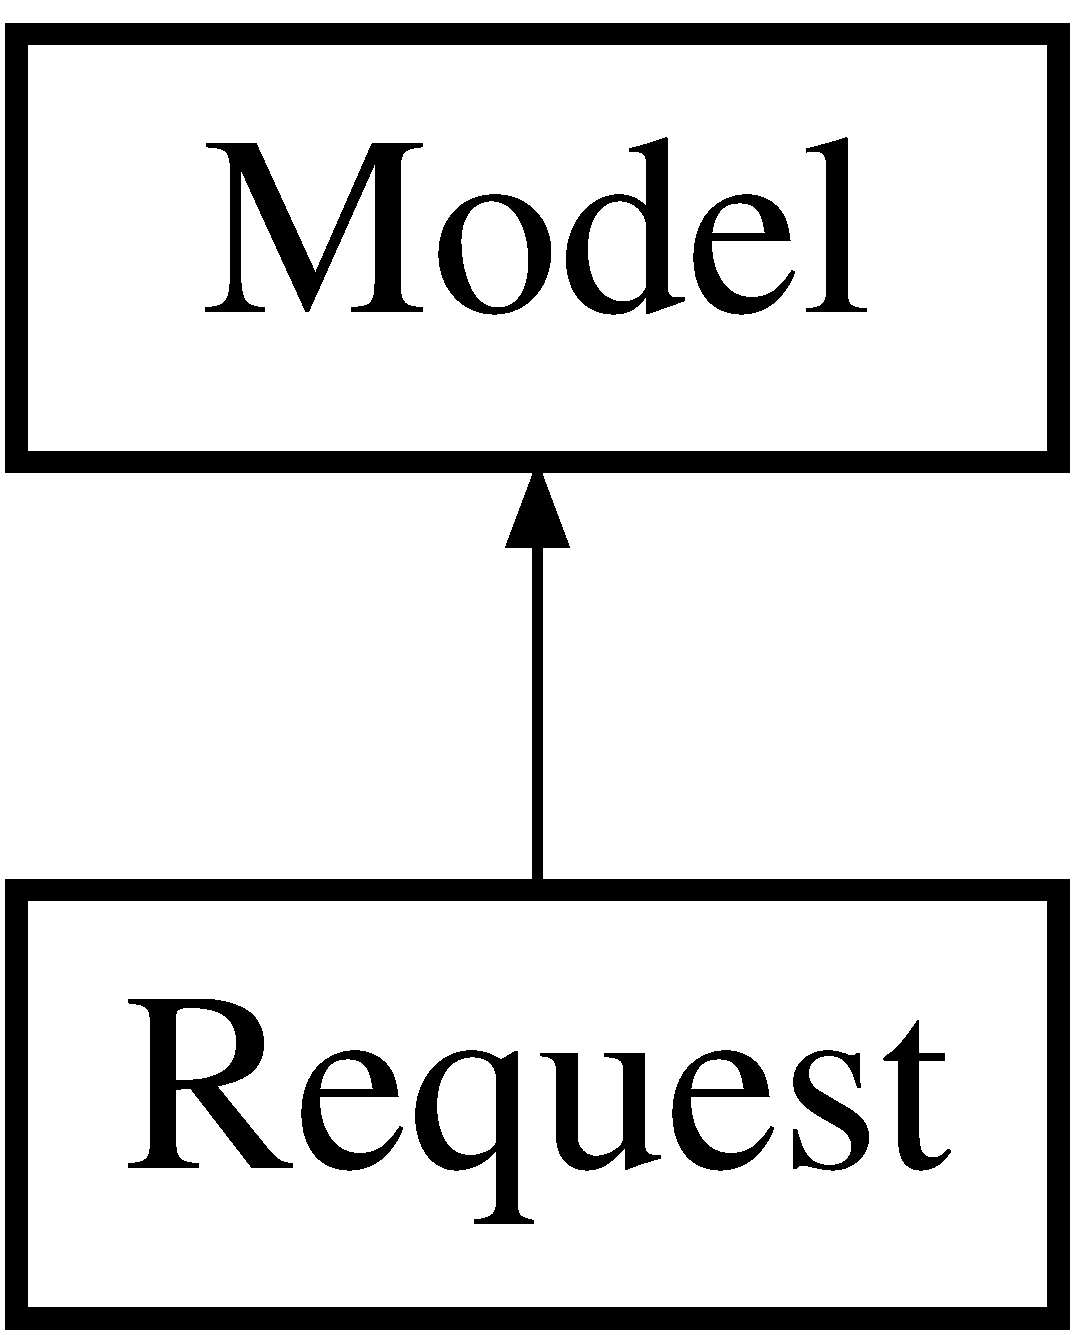
\includegraphics[height=2.000000cm]{classapp_1_1models_1_1_request}
\end{center}
\end{figure}
\subsection*{Public Member Functions}
\begin{DoxyCompactItemize}
\item 
\hypertarget{classapp_1_1models_1_1_request_a17dba92d96b9dd48c62f3ede3eef94d4}{}\label{classapp_1_1models_1_1_request_a17dba92d96b9dd48c62f3ede3eef94d4} 
{\bfseries rules} ()
\item 
\hypertarget{classapp_1_1models_1_1_request_afd2e4b9f8bf18ff12e1c13c06fd0438d}{}\label{classapp_1_1models_1_1_request_afd2e4b9f8bf18ff12e1c13c06fd0438d} 
{\bfseries form\+Name} ()
\item 
\hypertarget{classapp_1_1models_1_1_request_a86ff2ea4ddd02e750ebe8bd5d9f48379}{}\label{classapp_1_1models_1_1_request_a86ff2ea4ddd02e750ebe8bd5d9f48379} 
{\bfseries delete\+Request} (\$order\+Id)
\item 
\hypertarget{classapp_1_1models_1_1_request_a58129bfbc9df262c1757526d7121b2c7}{}\label{classapp_1_1models_1_1_request_a58129bfbc9df262c1757526d7121b2c7} 
{\bfseries add\+Request} (\$order\+Id=null)
\item 
\hypertarget{classapp_1_1models_1_1_request_a8dcfe595ca96111a0f58b12332e91297}{}\label{classapp_1_1models_1_1_request_a8dcfe595ca96111a0f58b12332e91297} 
{\bfseries count\+User\+Orders\+Requests} (\$user\+Id=null)
\item 
\hypertarget{classapp_1_1models_1_1_request_a81f5f30c06165ad677a6978177574efd}{}\label{classapp_1_1models_1_1_request_a81f5f30c06165ad677a6978177574efd} 
{\bfseries get\+Request\+By\+Id} (\$request\+Id)
\item 
\hypertarget{classapp_1_1models_1_1_request_aed483cb315b9fe576b5bf7853689b9fb}{}\label{classapp_1_1models_1_1_request_aed483cb315b9fe576b5bf7853689b9fb} 
{\bfseries confirm\+Reverse\+Request} (\$order\+Id)
\item 
\hypertarget{classapp_1_1models_1_1_request_ab35658a1ab9d6808c7ff60b9aff503a3}{}\label{classapp_1_1models_1_1_request_ab35658a1ab9d6808c7ff60b9aff503a3} 
{\bfseries get\+Requests\+By\+Order\+Id} (\$order\+Id)
\item 
\hypertarget{classapp_1_1models_1_1_request_ae6438ea0f721834fd79d06a6b135bced}{}\label{classapp_1_1models_1_1_request_ae6438ea0f721834fd79d06a6b135bced} 
{\bfseries confirm\+Request} (\$request\+Id)
\item 
\hypertarget{classapp_1_1models_1_1_request_ad5079a9fec1cf2c9f0c47e26f2cd594a}{}\label{classapp_1_1models_1_1_request_ad5079a9fec1cf2c9f0c47e26f2cd594a} 
{\bfseries is\+Request\+Confirmed} (\$order\+Id, \$user\+Id=null)
\item 
\hypertarget{classapp_1_1models_1_1_request_ac9cda0a12c6277fb0944cd84a38030f6}{}\label{classapp_1_1models_1_1_request_ac9cda0a12c6277fb0944cd84a38030f6} 
{\bfseries is\+Reverse\+Request\+Send} (\$order\+Id)
\item 
\hypertarget{classapp_1_1models_1_1_request_aa2845cbee688b64cf54571e1ed9d344b}{}\label{classapp_1_1models_1_1_request_aa2845cbee688b64cf54571e1ed9d344b} 
{\bfseries is\+Reverse\+Request\+Confirmed} (\$order\+Id, \$user\+Id=null)
\item 
\hypertarget{classapp_1_1models_1_1_request_a855fc1d62fe52310960b5c548e0ba696}{}\label{classapp_1_1models_1_1_request_a855fc1d62fe52310960b5c548e0ba696} 
{\bfseries deny\+Request} (\$request\+Id)
\end{DoxyCompactItemize}
\subsection*{Static Public Member Functions}
\begin{DoxyCompactItemize}
\item 
\hypertarget{classapp_1_1models_1_1_request_acb49a1e6d0325d6ff630aa0c942e9d5e}{}\label{classapp_1_1models_1_1_request_acb49a1e6d0325d6ff630aa0c942e9d5e} 
static {\bfseries has\+User\+Request} (\$order\+Id)
\end{DoxyCompactItemize}
\subsection*{Data Fields}
\begin{DoxyCompactItemize}
\item 
\hypertarget{classapp_1_1models_1_1_request_ae97941710d863131c700f069b109991e}{}\label{classapp_1_1models_1_1_request_ae97941710d863131c700f069b109991e} 
{\bfseries \$id}
\item 
\hypertarget{classapp_1_1models_1_1_request_a2b632c2ffbf6f86208b22492b86fa1c1}{}\label{classapp_1_1models_1_1_request_a2b632c2ffbf6f86208b22492b86fa1c1} 
{\bfseries \$order\+Id}
\item 
\hypertarget{classapp_1_1models_1_1_request_a84651f4070d04080f6c5fd3c98cc9104}{}\label{classapp_1_1models_1_1_request_a84651f4070d04080f6c5fd3c98cc9104} 
{\bfseries \$user\+Id}
\item 
\hypertarget{classapp_1_1models_1_1_request_afc31993e855f9631572adfedcfe6f34b}{}\label{classapp_1_1models_1_1_request_afc31993e855f9631572adfedcfe6f34b} 
{\bfseries \$login}
\item 
\hypertarget{classapp_1_1models_1_1_request_a87b032cba06009e3467abf1c8018d960}{}\label{classapp_1_1models_1_1_request_a87b032cba06009e3467abf1c8018d960} 
{\bfseries \$description}
\item 
\hypertarget{classapp_1_1models_1_1_request_a01cea456eabd700254653d5b8dcaba9d}{}\label{classapp_1_1models_1_1_request_a01cea456eabd700254653d5b8dcaba9d} 
{\bfseries \$time\+Posted}
\item 
\hypertarget{classapp_1_1models_1_1_request_a58391ea75f2d29d5d708d7050b641c33}{}\label{classapp_1_1models_1_1_request_a58391ea75f2d29d5d708d7050b641c33} 
{\bfseries \$status}
\end{DoxyCompactItemize}


The documentation for this class was generated from the following file\+:\begin{DoxyCompactItemize}
\item 
Request.\+php\end{DoxyCompactItemize}

\hypertarget{classapp_1_1models_1_1_user}{}\section{User Class Reference}
\label{classapp_1_1models_1_1_user}\index{User@{User}}
Inheritance diagram for User\+:\begin{figure}[H]
\begin{center}
\leavevmode
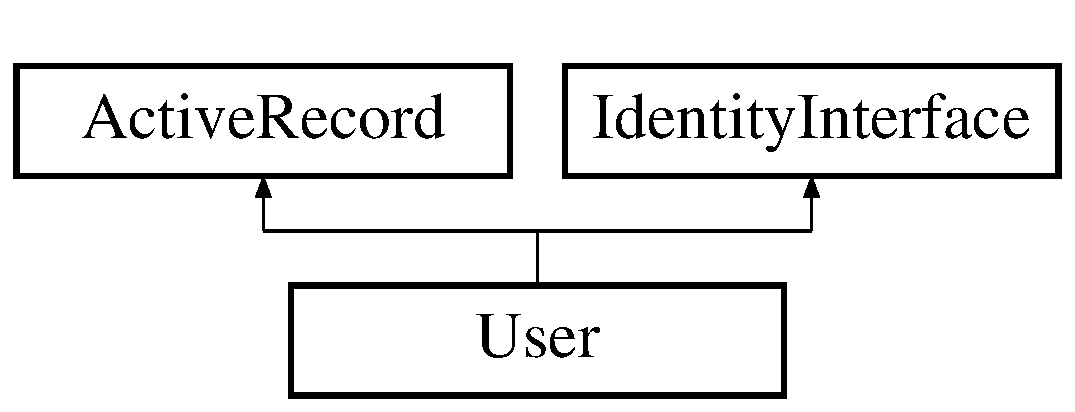
\includegraphics[height=2.000000cm]{classapp_1_1models_1_1_user}
\end{center}
\end{figure}
\subsection*{Public Member Functions}
\begin{DoxyCompactItemize}
\item 
\hypertarget{classapp_1_1models_1_1_user_a46794631cd74bd5fd20eedf24ac938d4}{}\label{classapp_1_1models_1_1_user_a46794631cd74bd5fd20eedf24ac938d4} 
{\bfseries get\+Orders} ()
\item 
\hypertarget{classapp_1_1models_1_1_user_adb49d249de40ebb2d6ef60cf2f4bcab3}{}\label{classapp_1_1models_1_1_user_adb49d249de40ebb2d6ef60cf2f4bcab3} 
{\bfseries get\+Posted\+Comments} ()
\item 
\hypertarget{classapp_1_1models_1_1_user_af3034ead082330d2c046a69814009808}{}\label{classapp_1_1models_1_1_user_af3034ead082330d2c046a69814009808} 
{\bfseries get\+Comments} ()
\item 
\hypertarget{classapp_1_1models_1_1_user_aae54d2938df6eac42a9a9020a64ae31b}{}\label{classapp_1_1models_1_1_user_aae54d2938df6eac42a9a9020a64ae31b} 
{\bfseries attribute\+Labels} ()
\item 
\hypertarget{classapp_1_1models_1_1_user_a3e35c8d3dbb2c513c618a664389e0926}{}\label{classapp_1_1models_1_1_user_a3e35c8d3dbb2c513c618a664389e0926} 
{\bfseries set\+Password} (\$password)
\item 
\hypertarget{classapp_1_1models_1_1_user_af86ba25ce1d7339d53bf28828aa3b29e}{}\label{classapp_1_1models_1_1_user_af86ba25ce1d7339d53bf28828aa3b29e} 
{\bfseries set\+Auth\+Key} ()
\item 
\hyperlink{classapp_1_1models_1_1_user_a12251d0c022e9e21c137a105ff683f13}{get\+Id} ()
\item 
\hypertarget{classapp_1_1models_1_1_user_ae9ca906fce6e9fe5fab3a6b42209d6a1}{}\label{classapp_1_1models_1_1_user_ae9ca906fce6e9fe5fab3a6b42209d6a1} 
{\bfseries get\+City} ()
\item 
\hyperlink{classapp_1_1models_1_1_user_a16828b12b5cf4522cb93f64c2b1af43b}{get\+Auth\+Key} ()
\item 
\hyperlink{classapp_1_1models_1_1_user_a54be63849d3e4d8db0fd23142cbc2a69}{validate\+Auth\+Key} (\$auth\+Key)
\item 
\hyperlink{classapp_1_1models_1_1_user_a179b92fbda1d7688a44cdcebf0b50e3f}{validate\+Password} (\$password)
\end{DoxyCompactItemize}
\subsection*{Static Public Member Functions}
\begin{DoxyCompactItemize}
\item 
static \hyperlink{classapp_1_1models_1_1_user_aa538c6278f56cff99f77d33cd6cb6981}{tablename} ()
\item 
\hypertarget{classapp_1_1models_1_1_user_a1c92c569609f0bcd1c10354de203c3b1}{}\label{classapp_1_1models_1_1_user_a1c92c569609f0bcd1c10354de203c3b1} 
static {\bfseries find\+Identity} (\$id)
\item 
static \hyperlink{classapp_1_1models_1_1_user_a38e0c72af43ac43dc7b789b796c27319}{find\+Identity\+By\+Access\+Token} (\$token, \$type=null)
\item 
static \hyperlink{classapp_1_1models_1_1_user_a168855925aeb48abecf006aff998fa52}{find\+By\+Username} (\$username)
\item 
\hypertarget{classapp_1_1models_1_1_user_a7f3bfa9dce7ff8fe55dc6cd84aec1d3e}{}\label{classapp_1_1models_1_1_user_a7f3bfa9dce7ff8fe55dc6cd84aec1d3e} 
static {\bfseries get\+Login\+By\+Userid} (\$id)
\item 
\hypertarget{classapp_1_1models_1_1_user_a8bb21f88e8a853e6b87733e38310515b}{}\label{classapp_1_1models_1_1_user_a8bb21f88e8a853e6b87733e38310515b} 
static {\bfseries city\+Change} (\$id, \$city)
\end{DoxyCompactItemize}


\subsection{Member Function Documentation}
\hypertarget{classapp_1_1models_1_1_user_a168855925aeb48abecf006aff998fa52}{}\label{classapp_1_1models_1_1_user_a168855925aeb48abecf006aff998fa52} 
\index{app\+::models\+::\+User@{app\+::models\+::\+User}!find\+By\+Username@{find\+By\+Username}}
\index{find\+By\+Username@{find\+By\+Username}!app\+::models\+::\+User@{app\+::models\+::\+User}}
\subsubsection{\texorpdfstring{find\+By\+Username()}{findByUsername()}}
{\footnotesize\ttfamily static find\+By\+Username (\begin{DoxyParamCaption}\item[{}]{\$username }\end{DoxyParamCaption})\hspace{0.3cm}{\ttfamily [static]}}

Finds user by username


\begin{DoxyParams}[1]{Parameters}
string & {\em \$username} & \\
\hline
\end{DoxyParams}
\begin{DoxyReturn}{Returns}
static$\vert$null 
\end{DoxyReturn}
\hypertarget{classapp_1_1models_1_1_user_a38e0c72af43ac43dc7b789b796c27319}{}\label{classapp_1_1models_1_1_user_a38e0c72af43ac43dc7b789b796c27319} 
\index{app\+::models\+::\+User@{app\+::models\+::\+User}!find\+Identity\+By\+Access\+Token@{find\+Identity\+By\+Access\+Token}}
\index{find\+Identity\+By\+Access\+Token@{find\+Identity\+By\+Access\+Token}!app\+::models\+::\+User@{app\+::models\+::\+User}}
\subsubsection{\texorpdfstring{find\+Identity\+By\+Access\+Token()}{findIdentityByAccessToken()}}
{\footnotesize\ttfamily static find\+Identity\+By\+Access\+Token (\begin{DoxyParamCaption}\item[{}]{\$token,  }\item[{}]{\$type = {\ttfamily null} }\end{DoxyParamCaption})\hspace{0.3cm}{\ttfamily [static]}}

\hypertarget{classapp_1_1models_1_1_user_a16828b12b5cf4522cb93f64c2b1af43b}{}\label{classapp_1_1models_1_1_user_a16828b12b5cf4522cb93f64c2b1af43b} 
\index{app\+::models\+::\+User@{app\+::models\+::\+User}!get\+Auth\+Key@{get\+Auth\+Key}}
\index{get\+Auth\+Key@{get\+Auth\+Key}!app\+::models\+::\+User@{app\+::models\+::\+User}}
\subsubsection{\texorpdfstring{get\+Auth\+Key()}{getAuthKey()}}
{\footnotesize\ttfamily get\+Auth\+Key (\begin{DoxyParamCaption}{ }\end{DoxyParamCaption})}

\hypertarget{classapp_1_1models_1_1_user_a12251d0c022e9e21c137a105ff683f13}{}\label{classapp_1_1models_1_1_user_a12251d0c022e9e21c137a105ff683f13} 
\index{app\+::models\+::\+User@{app\+::models\+::\+User}!get\+Id@{get\+Id}}
\index{get\+Id@{get\+Id}!app\+::models\+::\+User@{app\+::models\+::\+User}}
\subsubsection{\texorpdfstring{get\+Id()}{getId()}}
{\footnotesize\ttfamily get\+Id (\begin{DoxyParamCaption}{ }\end{DoxyParamCaption})}

\hypertarget{classapp_1_1models_1_1_user_aa538c6278f56cff99f77d33cd6cb6981}{}\label{classapp_1_1models_1_1_user_aa538c6278f56cff99f77d33cd6cb6981} 
\index{app\+::models\+::\+User@{app\+::models\+::\+User}!tablename@{tablename}}
\index{tablename@{tablename}!app\+::models\+::\+User@{app\+::models\+::\+User}}
\subsubsection{\texorpdfstring{tablename()}{tablename()}}
{\footnotesize\ttfamily static tablename (\begin{DoxyParamCaption}{ }\end{DoxyParamCaption})\hspace{0.3cm}{\ttfamily [static]}}

\hypertarget{classapp_1_1models_1_1_user_a54be63849d3e4d8db0fd23142cbc2a69}{}\label{classapp_1_1models_1_1_user_a54be63849d3e4d8db0fd23142cbc2a69} 
\index{app\+::models\+::\+User@{app\+::models\+::\+User}!validate\+Auth\+Key@{validate\+Auth\+Key}}
\index{validate\+Auth\+Key@{validate\+Auth\+Key}!app\+::models\+::\+User@{app\+::models\+::\+User}}
\subsubsection{\texorpdfstring{validate\+Auth\+Key()}{validateAuthKey()}}
{\footnotesize\ttfamily validate\+Auth\+Key (\begin{DoxyParamCaption}\item[{}]{\$auth\+Key }\end{DoxyParamCaption})}

\hypertarget{classapp_1_1models_1_1_user_a179b92fbda1d7688a44cdcebf0b50e3f}{}\label{classapp_1_1models_1_1_user_a179b92fbda1d7688a44cdcebf0b50e3f} 
\index{app\+::models\+::\+User@{app\+::models\+::\+User}!validate\+Password@{validate\+Password}}
\index{validate\+Password@{validate\+Password}!app\+::models\+::\+User@{app\+::models\+::\+User}}
\subsubsection{\texorpdfstring{validate\+Password()}{validatePassword()}}
{\footnotesize\ttfamily validate\+Password (\begin{DoxyParamCaption}\item[{}]{\$password }\end{DoxyParamCaption})}

Validates password


\begin{DoxyParams}[1]{Parameters}
string & {\em \$password} & password to validate \\
\hline
\end{DoxyParams}
\begin{DoxyReturn}{Returns}
boolean if password provided is valid for current user 
\end{DoxyReturn}


The documentation for this class was generated from the following file\+:\begin{DoxyCompactItemize}
\item 
User.\+php\end{DoxyCompactItemize}

%--- End generated contents ---

% Index
\backmatter
\newpage
\phantomsection
\clearemptydoublepage
\addcontentsline{toc}{chapter}{Index}
\printindex

\end{document}
